% \documentclass[a4paper,11pt]{amsart}
% \documentclass[11pt, twocolumn]{article}
\documentclass[
    a4paper, aps, twocolumn, floatfix, superscriptaddress,
    nofootinbib]{revtex4-1}
%\documentclass[a4paper,11pt]{report}

% \usepackage{pgfplots, mathpazo}
\usepackage{pgfplotstable}
\usepackage[utf8]{inputenc}
\usepackage{amsmath}
\usepackage{amssymb}
%\usepackage[document]{ragged2e}
\usepackage{hyperref}
\usepackage{cleveref}
\usepackage{amsmath}
\usepackage{listings}
\usepackage{xcolor}
\usepackage{graphicx}
\usepackage{float}
\usepackage{siunitx}
\usepackage{physics}
\usepackage{multirow}
\usepackage{booktabs}
\usepackage{indentfirst}
\usepackage{svg}
\usepackage[toc,page]{appendix}

\usepackage{titlesec} % Allows customization of titles
\renewcommand\thesection{\Roman{section}} % Roman numerals for the sections
\renewcommand{\thesubsection}{\Alph{subsection}} % Arabic numerals for the subsections
\titleformat{\section}[block]{\Large\scshape\centering\bfseries}{\thesection.}{1em}{} % Change the look of the section titles
\titleformat{\subsection}{\normalfont\large\filcenter\bfseries}{\thesubsection.}{1em}{}
\titleformat{\subsubsection}[runin]{\medium\bfseries}{\thesubsubsection.}{1em}{}% Change the look of the section titles
\usepackage{tikz}

\newcommand{\tikzmark}[2]{
    \tikz[overlay,remember picture,baseline] 
    \node[anchor=base] (#1) {$#2$};
}

% \usepackage{biblatex}

% \bibliography{references}
% \addbibresource{references.bib}


% \title[Variational Monte Carlo]{FYS4411 - Computational physics II: Quantum Mechanical Systems\\ Project 1: \\ Simulation of hard-sphere Bose gas using variational Monte Carlo}
% \author[Christensen, Fossheim]{Elisabeth Christensen and Håkon Dalyan Fossheim}
% \date{\today}

\title{}
\usepackage[backend=biber]{biblatex}
\addbibresource{references.bib}
% recommended:
% \usepackage{booktabs}
% \usepackage{array}
% \usepackage{colortbl}



% Colour scheme, see https://tex.stackexchange.com/a/119184/128247
\usepgfplotslibrary{colorbrewer}
\pgfplotsset{cycle list/Dark2}

\pgfplotstableset{
    every head row/.style={before row=\toprule,after row=\midrule},
    every last row/.style={after row=\bottomrule}
}
% \usepackage{multicol}

\begin{document}
% \begin{multicols}{2}


{\setlength\doublerulesep{5pt}}   %%<-- sep between consecutive rules

\begin{titlepage}

\newcommand{\HRule}{\rule{\linewidth}{0.5mm}} % Defines a new command for the horizontal lines, change thickness here

\center % Center everything on the page
 
%----------------------------------------------------------------------------------------
%	HEADING SECTIONS
%----------------------------------------------------------------------------------------

\textsc{\LARGE University of Oslo}\\[1.5cm] % Name of your university/college
\textsc{\Large FYS4411}\\[0.5cm] % Major heading such as course name
\textsc{\large Computational physics II: Quantum Mechanical Systems}\\[0.5cm] % Minor heading such as course title

%----------------------------------------------------------------------------------------
%	TITLE SECTION
%----------------------------------------------------------------------------------------

\HRule \\[0.4cm]
{ \huge \bfseries Project 1: \\ Simulation of hard-sphere Bose gas using Variational Monte Carlo}\\[0.4cm] % Title of your document
\HRule \\[1.5cm]
 
%----------------------------------------------------------------------------------------
%	AUTHOR SECTION
%----------------------------------------------------------------------------------------

\begin{minipage}{0.4\textwidth}
\begin{flushleft} \large
\emph{Author:}\\
Elisabeth \textsc{Christensen} % Your name
\end{flushleft}
\end{minipage}
~
\begin{minipage}{0.4\textwidth}
\begin{flushright} \large
\emph{Author:} \\
Håkon \textsc{D. Fossheim} % Supervisor's Name
\end{flushright}

\end{minipage}\\[2cm]

% If you don't want a supervisor, uncomment the two lines below and remove the section above
%\Large \emph{Author:}\\
%John \textsc{Smith}\\[3cm] % Your name

%----------------------------------------------------------------------------------------
%	DATE SECTION
%----------------------------------------------------------------------------------------

{\large \today}\\[2cm] % Date, change the \today to a set date if you want to be precise

%----------------------------------------------------------------------------------------
%	LOGO SECTION
%----------------------------------------------------------------------------------------

%\includegraphics{logo.png}\\[1cm] % Include a department/university logo - this will require the graphicx package
 
%----------------------------------------------------------------------------------------

\begin{abstract}
In this project we apply the variational Monte Carlo method to find the ground state of a dilute hard-sphere bose gas trapped in a harmonic potential. The method is first tested against the closed-form expression for a non-interacting system with a spherically symmetric potential by use of both the Metropolis algorithm and the Metropolis-Hastings algorithm. It is then expanded to include two-body interactions in an elliptical potential by use of the Metropolis algorithm alone. This is done in one, two and three dimensions for up to 500 particles. Due to correlated measurements, the blocking method is applied in order to present a proper error analysis. The optimal variational parameter for the trial wavefunction is calculated analytically to be $\alpha = 0.5$ for the non-interacting spherically symmetric system. No closed-form solution is obtainable for the elliptical system and so we resort to the steepest descent method to find the value of $\alpha$ that minimizes local energy. Lastly, we plot the one-body density of the interacting and non-interacting system and find that it qualitatively fits our theoretical model. 
\end{abstract}

\maketitle

\end{titlepage}


%\maketitle
\vfill


\newpage
% \tableofcontents{}

%----------------------------------------------------------------------
%   INTRODUCTION SECTION    
%----------------------------------------------------------------------
\section{Introduction}
A Bose-Einstein condensate is a state of matter achieved by cooling spin-1 particles, viz. bosons, to very low temperatures, causing them to "condense" into the lowest accessible quantum state. Here we present an upper bound for this ground state for a bose gas consisting of alkali atoms confined in a magnetic trap. We do so using a method known as \textit{Variational Monte Carlo}.

Variational Monte Carlo is a computational method utilizing the Monte Carlo algorithm combined with the variational principle from quantum mechanics to approximate an upper bound on the ground state energy of a system. We will compute this through mainly two algorithms: the Standard Metropolis and the Metropolis-Hastings algorithm. Furthermore, by building on the algorithms mentioned, we can develop a more complex quantum mechanical system consisting of either interacting or non-interacting bosons in a coordinate system of our choosing.

The variational principle relies heavily on the wavefunction necessary to describe our system, i.e. the Hamiltonian. Now, if we're clever about it, we can make an educated guess which allows us to find a normalized trial wavefunction that describes our system fairly well. However, by still making some room for adjustments, we can reach an even lower upper bound on the ground state energy if need be. This can be done by introducing a variational parameter, thereby the name variational principle.

But what if we don't want to go through all possible values for our variational parameter by hand? Well, that's easy, we can just include values that will ensure to \textit{minimize} our energy. Computationally, we can perform a gradient descent, converging into the most optimal parameter for the \textit{tightest} bound on the expectation value of the energy.

We can see the effects of interacting bosons vs. non-interacting bosons by studying the one-body density in an ellipsoidal system. We will lastly compare these effects to that of an ideal, i.e. spherical, system.


%----------------------------------------------------------------------
%   THEORY SECTION
%----------------------------------------------------------------------
\section{Theory}\label{sec:Theory}
\subsection{Variational Monte Carlo}
When dealing with complicated, intricate systems, such as many-body quantum mechanical problems, we often encounter large integrals concerning the behaviour of the objects within the system. An example of this, which will be the main focus of our report, is the expectation value of a given operator $\hat{O}$ when considering a system consisting of $N$ particles dependent on a wavefunction $\Psi$,

\begin{equation}\label{eq:1}
    \langle\hat{O}\rangle = \frac{\int d\bold r_1 d\bold r_2 ... d\bold r_N \Psi^\dagger(\bold r_1, \bold r_2, ..., \bold r_N)\hat{O}\Psi(\bold r_1, \bold r_2, ..., \bold r_N)}{\int d\bold r_1 d\bold r_2 ... d\bold r_N \Psi^\dagger(\bold r_1, \bold r_2, ..., \bold r_N)\Psi(\bold r_1, \bold r_2, ..., \bold r_N)}.
\end{equation}

Replacing the arbitrary quantum mechanical operator $\hat{O}$ with the more concrete operator $\hat{H}$, i.e. the Hamiltonian of the system, we can find the expectation value of the ground state energy. However, what if the exact form of the wavefunction is unknown? This is where the variational principle comes into play, as it allows us to find the \textit{upper bound} for the ground state energy of a system. That is, we guess a form of the wavefunction which satisfies the criteria to the system in question, and calculate the ground state energy, $E_{gs}$, as a function of the Hamiltonian. This is what we will apply to our system of the hard-sphere Bose gas. The variational principle is based on the claim that
\begin{align}
E_{gs} \leq \bra{\Psi_T}\hat{H}\ket{\Psi_T} \equiv \langle \hat{H} \rangle \label{eq:E_ground_state_var},
\end{align}
where $\Psi_T$ is the trial wavefunction and is considered to be normalised. The Hamiltonian can be expressed as
\begin{align}
    \hat{H} = \sum_i^N\left(-\frac{\hbar^2}{2m}\nabla_i^2 + V_{onebody}(\bold{r}_i)\right) + \sum_{i<j}^N V_{int}(\bold{r}_i, \bold{r}_j). \label{eq:Hamiltonian}
\end{align}

\subsubsection{Local energy} From the definitions of the Hamiltonian and the trial wavefunction we can declare a new operator $\hat{E}_L$, also known as the local energy,
\begin{align}
    \hat{E}_L(\bold r; \alpha) = \frac{1}{\Psi_T(\bold r; \alpha)}\hat{H}\Psi_T(\bold r; \alpha). \label{eq:local_energy}
\end{align}
The expected value of the local energy can be found by multiplying the integrand in the numerator of eq, \eqref{eq:1} by $\Psi/\Psi$: 
\begin{align}
    \langle \hat{H} \rangle &= \frac{\int d\bold r \Psi_T^\dagger(\bold r; \alpha) \Psi_T(\bold r; \alpha) \frac{1}{\Psi_T(\bold r; \alpha)} \hat{H} \Psi_T(\bold r; \alpha)}{\int d\bold r \Psi_T^\dagger(\bold r; \alpha) \Psi_T(\bold r; \alpha)}\\
    &= \frac{\int d\bold r E_L(\bold r; \alpha) |\Psi_T(\bold r; \alpha)|^2}{\int d\bold r |\Psi_T(\bold r; \alpha)|^2} = \langle \hat{E}_L \rangle
\end{align}
Which may be rewritten as 
\begin{equation}
    \langle \hat{E}_L \rangle = \int d\bold r E_L(\bold r; \alpha) \rho_T(\bold r; \alpha),
\end{equation}
where 
\begin{equation}\label{eq:7}
    \rho_T(\bold r; \alpha) = \frac{ |\Psi_T(\bold r; \alpha)|^2}{\int d\bold r |\Psi_T(\bold r; \alpha)|^2}.
\end{equation}
Finding a closed-form expression for $\langle \hat{E}_L \rangle$ is in general not possible when dealing with interacting many-body systems. One must therefore resort to numerical integration. For a fixed step length, the truncation error in integration methods based on Taylor expansion goes as $N^{-k/d}$ where $N$ is the number of grid points,  $d$ is the dimensionality of the system and $k \geq 1$ is an integer that depends on the method of choice. If we want to go from a  one dimensional integral to a $d$ dimensional one whilst keeping the truncation error fixed, we must compensate by increasing the number of grid points by a factor of $N^{(d-1)}$. This quickly results in absurd run-times.
In contrast, the truncation error in Monte Carlo integration scales as $\sigma \sim 1/\sqrt{N}$ for all dimensions. 

The idea behind Monte Carlo integration is to estimate the integral by taking the sum of a large set of samples randomly distributed in phase-space with weights corresponding to the underlying PDF
\begin{equation}\label{eq:8}
    \langle \hat{E}_L \rangle = \int d\bold r E_L(\bold r; \alpha) \rho(\bold r; \alpha) \approx  \sum_{i=1}^{N} E_L(\bold r; \alpha) \rho(\bold r; \alpha).
\end{equation}
Because we are unable to perform the integral in equation \eqref{eq:7} analytically, we do not know the normalization constant of the trial PDF. This is where the Metropolis algorithm comes to our rescue. We pick a random starting position and evaluate $E_L$. We then propose a new move in an arbitrary direction, and accept it if 
\begin{equation}
    1<\frac{\rho_T^{new}}{\rho_T^{old}}
\end{equation}
and reject it with a 50 \% probability otherwise.\footnote{See sections~\ref{subsubsec:brute-force} and~\ref{subsubsec:Metropolis-Hastings} under~\ref{sec:Methods}.~\nameref{sec:Methods} for further explanation on the methods used to achieve this computationally.} In this way, we can sample $E_L(\bold r; \alpha)$ directly from $\rho_T(\bold r; \alpha)$ without having to calculate the normalizaton constant. Now the likelyhood of getting a specific $E_L(\bold r; \alpha)$ is given by $\rho_T(\bold r; \alpha)$ and so there is no need for the weights in equation \eqref{eq:8}.
\begin{equation}
    \langle \hat{E}_L \rangle \approx \frac{1}{N} \sum_{i=1}^{N} E_L(\bold r; \alpha)
\end{equation}



\vspace{10}
Here, the wavefunction is dependent on a variational parameter $\alpha$, which allows us to experiment which wavefunction that will give us the best estimate on the minimal value of the local energy.

\subsection{Systems}
The system we will be focusing on throughout this report is that of a harmonic oscillator. From eq.~\eqref{eq:Hamiltonian} the external potential $V_{onebody}$ can then be expressed in the cases of a spherical (S) and an elliptical (E) harmonic trap as
\begin{align}
V_{onebody}(\bold{r}) = \begin{cases}
      \frac{1}{2}m\omega_{ho}^2r^2 & \text{(S)}\\
      \frac{1}{2}m[\omega_{ho}^2(x^2 + y^2) + \omega_z^2 z^2] & \text{(E)}
    \end{cases} \label{eq:V_ext}
\end{align}
where $\omega_{ho}^2$ is the trap potential strength. The repulsive potential $V_{int}$ is expressed as
\begin{align}
    V_{int}(|\bold{r}_i - \bold{r}_j| = \begin{cases}
    \infty &|\bold{r}_i - \bold r_j| \leq a \\
    0 & |\bold r_i - \bold r_j| > a
    \end{cases} \label{eq:V_int}
\end{align}
simulating the interaction between the particles. Here, $a$ is the hard-core diameter of the bosons, so that it is not possible for the bosons to penetrate each other.
\subsubsection{Trial wavefunction} The trial wavefunction must be able to satisfy the criteria following that of a harmonic oscillator. One criterion is that the wavefunction, including its derivative, must be well-defined at the origin. That is, at the boundary condition of when a boson approaches zero ($r_{i}\rightarrow 0$), the wavefunction must converge. In such a case, we can require that
\begin{align}
    \Psi_T \propto e^{-Zr_i}. \label{eq:psi_T_boundary_condition}
\end{align}

However, there is also the criterion of interaction between the particles, which can be incorporated in a so-called \textit{cusp} condition. In other words, we must take into consideration the distance $r_{ij}$ between the particles. The generalized trial wavefunction for $N$ particles can then be expressed as

\begin{align}
    &\Psi_T(\bold r) = \phi(\bold r_1)\phi(\bold r_2)...\phi(\bold r_N) \prod_{j<k}f(r_{jk}) \label{eq:trial_wavefunction_total}\\
    &= \left[\prod_i\exp[-\alpha(x_i^2 + y_i^2 + \beta z_i^2)]\right]\left[\prod_{j<k}f(a, |\bold r_j - \bold r_k|)\right]. \nonumber
\end{align}

Here, $\phi(\bold r_i)$ corresponds to the single-particle wavefunction of particle $i$ with a Gaussian shape. The product over $f(r_{jk})$ is also known as the Jastrow factor of the wavefunction, and takes into account the hard-sphere diameter of the bosons. This factor is expressed as

\begin{align}
    f(a, |\bold r_i - \bold r_j|) = \begin{cases}
    0 & |\bold r_i - \bold r_j| \leq a \\
    (1-\frac{a}{|\bold r_i - \bold r_j|}) & |\bold r_i - \bold r_j| > a
    \end{cases}
\end{align}

\subsubsection{Local energy} 
The analytic expression for the local energy for N non-interacting particles in $d$ dimensions can be deduced from the trial wavefunction and the Hamiltonian as defined above\footnote{See section~\ref{appendix:local_energy} under appendices for the derivation of this expression.}, i.e.
\begin{align}
    E_L(\bold r) &= \frac{1}{\Psi_T(\bold r)}\hat{H}\Psi_T \label{eq:E_local_analytic}\\
    &= \frac{1}{\Psi_T} \sum_i^N \left[\frac{-\hbar^2}{2m} 2\alpha(2\alpha \boldsymbol{r}_i^2 - d) \Psi_T + \frac{1}{2}m \omega_{ho}^2 \boldsymbol{r}_i^2 \Psi_T\right]. \nonumber
\end{align}

\subsubsection{Drift force}\label{subsubsec:drift_force}
The drift force $F$ as experienced by a particle can be expressed as the derivative of the trial wavefunction\footnote{See section~\ref{appendix:local_energy} under appendices for the derivation of eqs.~\eqref{eq:drift_force_non-interacting} and~\eqref{eq:double_derivative}.}, i.e.
\begin{align}
    F = \frac{2\nabla \Psi_T}{\Psi_T} = -4\alpha \boldsymbol{r}_i. \label{eq:drift_force_non-interacting}
\end{align}
While for the interacting case we have that the double derivative in~\eqref{eq:Hamiltonian}, when acting on the trial wavefunction, is
\begin{align}
    \frac{1}{\Psi_T(\vec r)} \nabla^{2}_{k} \Psi_{T}(\boldsymbol{r})  &=\frac{\nabla_k^2 \phi(\boldsymbol{r}_k)}{\phi(\boldsymbol{r}_k)} + 2\frac{\nabla_k \phi(\boldsymbol{r}_k)}{\phi(\boldsymbol{r}_k)} \sum_{j\neq k} \frac{\boldsymbol{r}_k-\boldsymbol{r}_j}{r_{kj}} u'(r_{kj})\label{eq:double_derivative} \\
    &+\sum_{i\neq k} \sum_{j \neq k} \frac{\left(\boldsymbol{r}_k - \boldsymbol{r}_i\right)\left(\boldsymbol{r}_k - \boldsymbol{r}_j\right)}{r_{ki} r_{kj}} u'(r_{ki}) u'(r_{kj})\nonumber\\
    &+\sum_{j\neq k}\left( u''(r_{kj}) + \frac{2}{r_{kj}}u'(r_{kj}) \right)\nonumber.
\end{align}
%The derivations for expressions~\eqref{eq:E_local_analytic},~\eqref{eq:drift_force_non-interacting} and~\eqref{eq:double_derivative} can be found in appendix A.

\subsubsection{One-Body Density}\label{subsubsec:one_body}
For a system of N particles, the one-body density of particle \boldsymbol{i} is 

\begin{equation}
    \rho(\boldsymbol{r}_i) = \int |\psi(\boldsymbol{r}_1,...,\boldsymbol{r}_{i},...,\boldsymbol{r}_{N})|^2 d\boldsymbol{r}_1 \cdots d\boldsymbol{r}_{i-1} d\boldsymbol{r}_{i+1} \cdots d\boldsymbol{r}_{N},
\end{equation}

and is the probability of finding particle \boldsymbol{i} within the volume $d\boldsymbol{r}_i^3$. The likelyhood of finding the particle anywhere is one, and so 

\begin{equation}
    \int \rho(\boldsymbol{r}_i) d\boldsymbol{r}_i^3 = 1.
\end{equation}

The one-body density is the same for every particle, and thus 
\begin{equation}\label{eq:21}
    \sum_{i=1}^{N}\int \rho(\boldsymbol{r}_i) d\boldsymbol{r}_i^3 =
    \int \rho(\boldsymbol{r}) d\boldsymbol{r}^3 =N
\end{equation}
where we defined $\rho(\boldsymbol{r}) \equiv \sum_{i=1}^N \rho(\boldsymbol{r}_i)$. 

In the case of an elliptical potential, the single particle wavefunction $\psi \propto e^{-\alpha(x^2+y^2+\beta z^2)}$ gives 
$\rho(\boldsymbol{r}) \propto e^{-2\alpha(x^2+y^2+\beta z^2)}$. $\rho(\boldsymbol{r})$ is therefore constant on the surfaces of ellipsoids. For $\beta >1$ the ellipsoids are oblate spheroids (disc-shaped) and for $\beta<1$, they are prolate spheroids (cigar-shaped). In either case, the following holds 
\begin{equation}
    x^2+y^2+\beta z^2 = R^2,
\end{equation}
where $R^2$ is the radius of the projection of the ellipsoid onto the xy-plane, i.e. $R^2 = (x^2+y^2)|_{z=0}$. We can then perform the integral in equation \eqref{eq:21} by integrating $\rho(R)$ with respect to ellipsoidal shells of thickness $dR$, see figure \ref{fig:1}. 

\begin{figure}[H]
\makebox[0.5\textwidth][c]{\includesvg[width=0.5\textwidth]{ellipsoidgrey.svg}}%
 \caption{}
 \label{fig:1}
\end{figure}
The volume of our ellipsoid is given by 
\begin{equation}\label{eq:ellipsoid_volume}
    V = \frac{4\pi}{3\sqrt{\beta}} R^3,
\end{equation}
and so 
\begin{equation}
    dV =\frac{4\pi}{3\sqrt{\beta}}\left((R+dR)^3-(R)^3 \right).
\end{equation}
Equation \eqref{eq:21} then becomes
\begin{equation}\label{eq:onebody_density_integral}
   N= \int \rho(\boldsymbol{r}) d\boldsymbol{r}^3 = \int_0^{\infty} \rho(R) dV. 
\end{equation}
We can discretize this integral. Let $R_{max}$ be large enough that $\rho(R_{max})$ is practically zero. For a chosen $\Delta R$, the number of bins is given by $M = R_{max}/\Delta R$, and so the discretized version of the integral is
\begin{equation}
    N \approx \sum_{i=0}^{M} \rho(R_i)  \Delta V_i,
\end{equation}
or 
\begin{equation}\label{eq:27}
    N_i \approx\rho(R_i) \Delta V_i,
\end{equation}
where $N_i$ is the number of particles in shell $i$, and 
\begin{equation}
    \Delta V_i =\frac{4\pi}{3\sqrt{\beta}}\left((R_i+\Delta R)^3-(R_i)^3 \right).
\end{equation}
We can rearrange equation \eqref{eq:27} to get the one-body density expressed in terms of variables we can easily extract from our Monte Carlo steps: 
\begin{equation}\label{eq:29}
   \rho(R_i)   \approx \frac{N_i}{\Delta V_i} = \frac{3\sqrt{\beta}}{4 \pi \left((R_i+\Delta R)^3-(R_i)^3 \right)} N_i
\end{equation}
Sampling $R_i$ for every particle in every Monte Carlo step and adding the expression in equation \eqref{eq:29} to the bin corresponding to $R_i$ yields a histogram. Normalizing this histogram by dividing each bin by the number of particles times the number of Monte Carlo steps gives us an  approximation of the one-body density $\rho(\boldsymbol{r})$. Note that in the spherically symmetric case we get the exact same equations, but with $\sqrt{\beta} = 1$.


\subsection{Statistical physics}
When performing a Monte Carlo sampling, one may be subject to both systematic and statistical errors. A possible source is that of the steplengths chosen for our system, which can lead to increasing nuisance parameters, such as the variance $\sigma^2$. So, let's look at the nuisance parameters necessary to tell us about the precision of our Monte Carlo sampling.

\subsubsection{Uncorrelated stochastic variables}
When dealing with Monte Carlo sampling we often draw random values, but by doing so at large scales the system can become predictable. In such a case, we can adjust the nuisance parameters to include stochastic variables within a certain sample size $n$. Thus, the sample mean can be expressed as
\begin{equation}%\label{eq:30}
    \Bar{x}_n \equiv \frac{1}{n} \sum_{k=1}^n x_k. \label{eq:uncorrelated_mean}
\end{equation}
% Let $X$ be the stochastic variable whose PDF is that of the measurements, and let $\overline{X}$ be the stochastic variable whose PDF is the same as the sample average.
The variance of the measurements is given by
\begin{equation}%\label{eq:31}
    \sigma^2 = \frac{1}{n}\sum_{i=1}^n (x_i - \Bar{x}_n)^2, \label{eq:uncorrelated_variance}
\end{equation}
 where we used $\bar{x}_n$ as an estimate of the true sample mean, $\mu$. The central limit theorem tells us that $\bar{x}_n$ approaches $\mu$ as the number of measurements goes to infinity.

 
Furthermore, the covariance of the measurements can be expressed as
\begin{equation}\label{eq:32}
    \text{cov}(x) \equiv \frac{1}{n} \sum_{kl} (x_k-\Bar{x}_n)(x_l-\Bar{x}_n),
\end{equation}
which for an uncorrelated set of measurements is just the variance given in eq.\eqref{eq:uncorrelated_variance}. 
To determine how well the sample mean approximates the true mean value, we can calculate the sample error, which is just the standard deviation of the sample mean itself. It turns out that the sample variance is related to the measurements in the following manner \cite{Stat.Phys.}
\begin{equation}\label{eq:33}
    \text{err}_{\overline{x}}^2 = \text{var}(\overline{x})= \frac{1}{n}\text{cov}(x). 
\end{equation}

\subsubsection{Serially correlated stochastic variables}
The Metropolis algorithm produces a time-series which is serially correlated, meaning that each measurement covaries with neighbouring measurements within a certain distance. We are interested in finding this "radius" of influence. From eq. \eqref{eq:33} and \eqref{eq:32}, we have
\begin{equation}
    \text{err}_{\overline{x}}^2 = \frac{1}{n} \text{cov}(x) = \frac{1}{n}\frac{1}{n}\sum_{kl}(x_k - \bar{x}_n) (x_l - \bar{x}_n).
\end{equation}
We may split the covariance into cross terms and terms where $x_k = x_l$. The latter terms just sum up to the variance, and so 
\begin{equation}
    \text{err}_{\overline{x}}^2 = \frac{1}{n} \text{var}(x) + \frac{1}{n}(\text{cov}(x)-\text{var}(x)).
\end{equation}
The cross terms sum over all pairwise combinations of $x_k$ and $x_l$ twice while excluding the terms where $x_k = x_l$. We therefore get 
\begin{equation}\label{eq:36}
    \text{err}_{\overline{x}}^2=\frac{1}{n^2} \sum_{k=1}^n (x_k - \Bar{x}_n)^2 + \frac{2}{n^2}\sum_{k<l}(x_k - \Bar{x}_n)(x_l-\Bar{x}_n).
\end{equation}
Denoting $(x_k - \bar{x}_n)(x_l - \bar{x}_n)$ by $\Tilde{x}_k\Tilde{x}_l$, the correlation term may be written as 
\begin{align}\label{eq:34}
    \sum_{k<l}  \Tilde{x}_k\Tilde{x}_l=\sum_{k=1}\sum_{l=k+1} \Tilde{x}_k\Tilde{x}_l& \\
    = \Tilde{x}_1\Tilde{x}_2+\Tilde{x}_1\Tilde{x}_3+\Tilde{x}_1\Tilde{x}_4+\Tilde{x}_1\Tilde{x}_5+...+\Tilde{x}_1\Tilde{x}_n& \nonumber \\
    + \Tilde{x}_2\Tilde{x}_3+\Tilde{x}_2\Tilde{x}_4+\Tilde{x}_2\Tilde{x}_5+...+\Tilde{x}_2\Tilde{x}_n& \nonumber \\
     + \Tilde{x}_{3}\Tilde{x}_{4}+\Tilde{x}_3\Tilde{x}_5 +...+ \Tilde{x}_{3}\Tilde{x}_{n}& \nonumber \\
     \ddots \qquad \qquad \vdots \qquad& \nonumber \\
    +\Tilde{x}_{n-1}\Tilde{x}_n \nonumber
\end{align}
This sum can be split up into its diagonal parts. As can be seen above, the samples in a given diagonal are all separated by a fixed distance $d$, with $d=1$ for the leftmost diagonal and $d=n-1$ for the rightmost one. The sum over a given diagonal $d$ is then 
\begin{equation}
     \sum_{k=1}^{n-d}\Tilde{x}_k \Tilde{x}_{k+d}.
\end{equation}
Now, defining 
\begin{equation}
    f_d = \frac{1}{n} \sum_{k=1}^{n-d} \Tilde{x}_k \Tilde{x}_{k+d}
\end{equation}
the correlation part of equation \eqref{eq:33} can be written as 
\begin{equation}
 \frac{2}{n^2} \sum_{k<l} \Tilde{x}_k \Tilde{x}_l = \frac{2}{n} \sum_{d=1}^{n-1} f_d   
\end{equation}
When $d=0$, $f_d$ is simply the variance. It is therefore natural to introduce the autocorrelation function
\begin{equation}
\kappa_d = \frac{f_d}{\text{var}(x)},
\end{equation}
which is always equal to 1 for $d=0$. The sample error can now be written as 
\begin{align}
    \text{err}^2 &= \frac{1}{n}\text{var}(x) + \frac{2}{n} \text{var}(x) \sum_{d=1}^{n-1} \frac{f_d}{\text{var}(x)}\\ 
    & = \frac{1}{n} \text{var}(x) \left( 1 + 2\sum_{d=1}^{n-1} \kappa_d \right).
\end{align}
Defining the autocorrelation time as 
\begin{equation}
\tau \equiv \left( 1 + 2\sum_{d=1}^{n-1} \kappa_d \right),
\end{equation}
the final expression for our sample error becomes 
\begin{equation}\label{eq:43}
    \text{err}_{\overline{x}}^2 = \frac{\tau}{n}\text{var}(x).
\end{equation}
The sample can be thought of as being reduced to effectively $n_{eff} = \frac{n}{\tau}$ measurements. 
When all the measurements are uncorrelated, $\tau = 1$ and the sample error is given by $\text{var}(x)/n$. For correlated samples, $\tau>1$ and so the error increases. This means that simply calculating the sample error with $\tau=1$ will in our case give a too low estimate of the error, since our measurements are correlated. We therefore need to find the autocorrelation time in order to find the true sample error. Doing this every time we run a Monte Carlo simulation by actually calculating $f_d$ would be very computationally expensive, as every measurement would have to be stored. In addition we would have to calculate the sum of $(n^2-n)/2$ products in order to evaluate $f_d$, which is no small task for $n \sim 10^7 $. 

Instead we can determine the autocorrelation time and the correct sample error through blocking. We calculate ${\text{err}}_X^2$ for each blocking transformation. When the error stops increasing and reaches a plateau, the last measurements of a block are no longer correlated with the first, and we can set this block size as the correlation time. The blocking procedure is described in more detail in section~\ref{subsubsec:blocking}.

% The samples of $\vec{X_i}$ are now uncorrelated in the sense that the $j$'th measurement of $(\vec{X_i})_{k+1}$ is independent of the $j$'th measurement of $(\vec{X_i})_{k}$. \cite{Jonsson}

%----------------------------------------------------------------------
%   METHODS SECTION
%----------------------------------------------------------------------
\section{Methods}\label{sec:Methods}
\subsection{Variational Monte Carlo}
\subsubsection{Standard Metropolis method}\label{subsubsec:brute-force}
When simulating the ground state energy of a trapped, hard-sphere Bose gas we can utilize a variational Monte Carlo method based on the Metropolis algorithm. Two requirements to a Markov process is that of detailed balance, i.e. a system which reaches equilibrium stays at equilibrium, and that of ergodicity in which the ensemble average equals the time average. Here, the Standard Metropolis algorithm satisfies both and can thus be used as a reliable option when modelling a system of both interacting and non-interacting bosons with a certain trial wavefunction \cite{notes}.

The Standard Metropolis algorithm, also known as \textit{brute force} Metropolis, is based on initializing the particles at a random location $x^i$ in space, with a uniform distribution. From that point on, we can suggest a move for each individual particle at a state $\mu$ to a new state $\nu$ with a certain transition probability $T(\mu\rightarrow \nu)$. If the ratio of transition probabilities ($T(\nu\rightarrow \mu)/T(\mu\rightarrow \nu)$) is higher than some tolerance $s$, of our choosing, then the move is accepted and the trial positions now become the current positions of our particles. If the ratio is lower than $s$, then the move is rejected, and the particles remain stationary at their original positions. In our case, the transition probabilities are based on the values generated by the wavefunction for each new state.

\subsubsection{Metropolis-Hastings method}\label{subsubsec:Metropolis-Hastings} When we are not dealing with a symmetric initial distribution of particles in the phase space, as is the assumption under the brute force Metropolis algorithm, we can make use of what is known as the Metropolis-Hastings algorithm, i.e. \textit{importance sampling}. Like the brute-force method, it is a Markov chain Monte Carlo method (MCMC) and utilises the same approach to calculate the acceptance or rejection of a move from one state $\mu$ to a new state $\nu$. But, there is a profound difference when considering the actual move to the new state. Here, one takes into account the time-evolution of the probability distribution function (PDF) of the velocities of the particles. The time-evolution is due to the particles experiencing a stochastic drift force $F$\footnote{See section~\ref{subsubsec:drift_force} under~\ref{sec:Theory}.~\nameref{sec:Theory} for a more thorough, theoretical explanation on the drift force, otherwise also known as the quantum force.} and can be expressed by the Fokker-Planck equation in eq.~\ref{eq:Fokker-Planck}. \\

\indent The total probability distribution function at three different times $t_0 < t' < t$, can be expressed by the Einstein-Smoluchenski-Kolmogorov-Chapman (ESKC) equation
\begin{align}
    W(\bold x, t | \bold x_0, t_0) = \int_{-\infty}^\infty W(\bold x, t | \bold x', t')W(\bold x', t' | \bold x_0, t_0)d\bold x', \label{eq:W_PDF}
\end{align}
and is derived from the three different probability functions at separate times $t_0$, $t'$, $t$, as defined below
\begin{align*}
    w(\bold x, t) &= \int_{-\infty}^\infty W(\bold x, t | \bold x', t') w(\bold x', t')d\bold x', \\
    w(\bold x, t) &= \int_{-\infty}^\infty W(\bold x, t | \bold x_0, t_0) w(\bold x_0, t_0)d\bold x_0, \\
    w(\bold x', t') &= \int_{-\infty}^\infty W(\bold x', t' | \bold x_0, t_0) w(\bold x_0, t_0)d\bold x_0.
\end{align*}
The time-evolution of the probability distribution function in~\eqref{eq:W_PDF} can be expressed as
\begin{align}
    \frac{\partial W(\bold x, s | \bold x_0)}{\partial s} = -\frac{\partial M_1 W(\bold x, s | \bold x_0)}{\partial x} + \frac{1}{2}\frac{\partial^2 M_2 W(\bold x, s | \bold x_0)}{\partial x^2} \label{eq:Fokker-Planck},
\end{align}
i.e. the Fokker-Planck equation. Here, $\bold x$ represents the spatial dependence, $s = t' - t_0$, and $x_0$ is the  position at time $t_0$.

The Langevin equation describes the stochastic drift force a particle is subject to as it moves throughout the medium, and is expressed as

\begin{align}
    \frac{dv}{dt} = -\xi v + F. \label{eq:Langevin}
\end{align}

Once these properties are taken into consideration, one can calculate the acceptance ratio by also taking into account the Green's function as a function of the quantum force experienced by a particle in the state $\mu$, and the quantum force experienced after the move to a new state $\nu$.

\subsection{Resampling methods}
\subsubsection{Bootstrap}\label{subsubsec:bootstrap}
The idea of the bootstrap method is as follows. We have a sample consisting of $n$ independent, identically distributed (i.i.d.) variables represented by the vector $\hat{x}$. Our goal is to find the PDF of some function of $\hat{x}$,  $\hat{\theta}(\hat{x})$. To find this PDF, we draw with replacement $n$ numbers from $\hat{x}$. Denote this vector of numbers by $\hat{x}^{\ast}$. Calculate $\hat\theta^{\ast}(\hat{x}^{\ast}) =\hat\theta(\hat{x}^{\ast})$ and repeat the process $n$ or less times. From this we can create a histogram of the relative frequency of $\hat\theta^{\ast}$, which is our estimate of the PDF. This is rarely done in practice, as one usually just calculates the quantity in interest with a point estimator.

In our case, we are interested in knowing the variance of the sample means. For a sample of size $n$, the bootstrap algorithm then tells us to draw  $n$ measurements with replacement from the same Monte Carlo sample and calculate the mean $\overline{x}^{\ast}$. Repeating this process $\sim n$ times, an estimate of the sample variance is found by use of eq.\eqref{eq:33}. This method works best for small samples. For larger sample sizes the complexity of the bootstrap method is deterring, not to mention that the measurements in our case aren't i.i.d.
\subsubsection{Blocking}\label{subsubsec:blocking}
% Since the Metropolis Algorithm only proposes new moves that are in the vicinity of the last one, more specifically within one step length of the current position, the measurements of a given Monte Carlo sample will be dependent on one another, i.e. correlated. When evaluating eq.~\eqref{eq:sigma_correlated} we must take into account the autocorrelation time $\tau$. The problem is however, that we do not know the correlation time. This is where the resampling method of blocking becomes useful.

In contrast to the bootstrap method, the blocking method works best for large sample sizes. Let the original sample contain $n=2^d$ measurements, where $d$ is an integer. In order to guarantee that the automation process introduced later in this section works, let's restrict ourselves to the case where these measurements form a stationary time series, which is the case when using the Metropolis algorithm. Denote this time series by the vector $\hat{X}$. The idea behind blocking is to perform so-called blocking transformations, which halves the length of the vector by taking the mean of two adjacent elements of the previous vector. Mathematically, a transformation $k$, where $k \in [1, 2, ..., d]$, is expressed as
\begin{align}
    &(\hat X_0)_k \equiv (\hat X)_k \nonumber\\
    &(\hat X_{i+1})_k \equiv \frac{1}{2}((\hat X_i)_{2k-1} + (\hat X_i)_{2k}). \label{eq:blocking_transformation}
\end{align}
% From these transformations, we can now compute the autocorrelation as described in eq.~\eqref{eq:autocorrelation}.
 It can be shown that if $\hat{X}_0$ is a stationary time series, then so is $\hat{X}_k$ \cite{Jonsson}. Now, we may treat each element/block of a given vector $\hat{X}_i$ as an estimate of the mean value of a Monte Carlo sample. For brevity, denote the elements of a given vector by $X_k$. We wish to find the variance of these elements/means for a given blocking iteration. Ignoring the blocking iteration index, the variance is given by \cite{Jonsson}
 \begin{equation}
     \text{var}(\overline{X}) = \text{var}\left(\frac{1}{n_k} \sum_{k=1}^{n_k} X_k \right) = \frac{1}{n_k^2} \text{cov}\left( \sum_{i=1}^{n_k} X_i, \sum_{j=1}^{n_k} X_j \right).
 \end{equation}
The autocovariance is defined as 
 \begin{equation}
     \gamma(h) = \text{cov}(X_i,X_{i+h}),
 \end{equation}
where $h = |i-j|$. From the distributive property of the covariance, we get 
 \begin{align}
     &\text{var}(\overline{X}) = \frac{1}{n_k^2}\sum_{i=1}^{n_k}\sum_{j=1}^{n_k} \text{cov}(X_i,X_j)\\ \nonumber
     & = \frac{1}{n_k^2}\Big[n_k\gamma(0) + (n_k-1)\gamma(1) + (n_k-2)\gamma(2)+...+\gamma(n_k-1)\\ \nonumber
     & + (n_k-1) \gamma(-1) + (n_k-2) \gamma(-2) +...+\gamma(1-n_k)\Big],
 \end{align}
where $\gamma(0)$ is just the sample variance with no consideration to correlation. Let's denote this variance by $\sigma_k^2$. This yields
\begin{align}
 \text{var}(\overline{X}) &= \frac{\sigma_k^2}{n_k} + \frac{2}{n_k^2} \sum_{h=1}^{n_k-1} (n_k-h)\gamma(h) \\
 &= \frac{\sigma_k^2}{n_k} + \underbrace{\frac{2}{n_k} \sum_{h=1}^{n_k-1}\left(1-\frac{h}{n_k} \right) \gamma(h)}_{e_k},
\end{align}
where $e_k$ is called the truncation error. It can be shown that \cite{Stat.Phys.}
 \begin{equation}
     \overline{X}_{j+1} = \overline{X}_{j},
 \end{equation}
 as one might expect. By induction one can then show that 
 \begin{equation}
     \text{var}(\overline{X}_0) = \text{var}(\overline{X}_i) = \text{var}(\overline{X}).
 \end{equation}
 The variance of the blocks is therefore constant as a function of blocking iteration $k$;
 \begin{equation}
     \text{var}(\overline{X}) = \frac{\sigma_k^2}{n_k} + e_k
 \end{equation}
 The sequence $\{e_k\}_{k=0}^{d-1}$ is decreasing \cite{Jonsson}, and thus $e_k$ can be made as small as we like by increasing $k$ through increasing $d$. For $\text{var}(\overline{X})$ to remain constant for each blocking iteration, $\frac{\sigma_k^2}{n_k}$  must increase as a function of $k$ and eventually reach a plateau when $e_k \approx 0$ and the blocks are no longer correlated. We can then extract the variance from one of these uncorrelated blocking iterations. 
 
 This can be done in a brute force manner by plotting $\sigma_k^2/n_k$ vs. $k$ and estimating when the plateau is reached, or one may automate this process. The automation procedure is explained in great detail in \cite{Stat.Phys.}. The outline is as follows: For each blocking iteration, calculate the test statistic $M_j$ given by 
 \begin{equation}
     M_j = \sum_{k=j}^{d-1}\frac{n_k\left[(n_k-1) \sigma_k^2/(n_k^2) \ \gamma_k(1) \right]}{\sigma_k^4}.
 \end{equation}
$M_j$ is $\chi^2$-distributed with $d-k$ degrees of freedom. Next, pick a significance level, $\alpha$, and find the smallest $k$ such that $M_k \leq q_{d-k}(1-\alpha)$. Using this $k$, the final estimate of the sample variance is $\sigma_b^2 = \sigma_k^2/n_k$.
 

\subsection{Optimization methods}
In order to achieve the minimum value of the local energy expressed in eq.~\eqref{eq:local_energy}, we can adjust the variational parameter $\alpha$ of the trial wavefunction in eq.~\eqref{eq:trial_wavefunction_total}. This can be done by multiple methods such as the conjugate gradient method, the steepest descent method or simply by Newton's method. In this project we will rely on the steepest descent method, computationally known as gradient descent (GD).
\subsubsection{Gradient descent}
When dealing with a differentiable function $F$ dependent on a variational parameter, we can find the local minimum by taking steps in the negative direction proportional to $-\nabla F$.\footnote{If we want the local maximum we may take steps in the positive direction proportional to $+\nabla F$.} Now, there is a certain learning curve as to how quickly we can reach a local minimum. This learning curve is dependent on the learning rate $\gamma$, often also referred to as the step length. The smaller the learning rate, the longer it takes to converge to an optimal value. The greater the learning rate the more prone we are to experience fluctuant behaviour.

The gradient descent method is based on an iterative scheme in which the next value, $x_{k+1}$, is dependent on the previous value $x_k$. This can also be expressed as
\begin{align}
    \bold x_{k+1} = \bold x_{k} - \gamma_k\nabla F(\bold x_k),
\end{align}
where we start off the sequence with an initial guess $x_0$. In our case, the differentiable function $F$ corresponds to the derivative of the local energy $E_L$ wrt. $\alpha$, whereas $x_k$ corresponds to the current value of $\alpha_k$.

One must however be aware of the limits of conjugate gradient methods, such as the gradient descent. For one, the gradient descent will converge to a minimum, but not necessarily the global minimum. In other words, it may get stuck in a local minimum unless we run the optimization method for a very long time, or choose a near perfect initial value $x_0$. And second, as mentioned earlier, it is dependent on the learning rate $\gamma_k$, and can thus become very slow if we want a higher accuracy in the optimal parameter.

%----------------------------------------------------------------------
%   RESULTS SECTION 
%----------------------------------------------------------------------
\section{Results}\label{sec:Results}
%********************************************
%   Non-interacting systems
%********************************************
\subsection{Non-interacting spherical system}
%*********************
%   Brute force
%*********************
\subsubsection{Standard Metropolis}
We start off by looking at the simplest case, i.e. examining the brute force Metropolis algorithm. By setting $\beta = 1$ and $a=0$ we will look at a spherical harmonic oscillator with no interaction. Table~\ref{tab:b_bruteforce_1part_3dim} shows the measurements of the local energy as a function of $\alpha$. Here, $\sigma$ corresponds to the biased sample error of the Monte Carlo runs, whereas $\sigma_b$ corresponds to the error produced by the blocking method. As we can see, $\sigma$ produces lower errors between the measurements than that of the blocking error, giving a misleading confidence in our results. The number of accepted steps is represented by the variable $A_{ratio}$, while $t_{CPU}$ tells us the amount of computational time required (in seconds) to calculate the local energy.

This computation is furthermore done for $N = 1$, 10 and 100 particles in both $d = 1$, 2 and 3 dimensions, as is visualized in figure~\ref{fig:brute_force_spherical_localE} showing the local energy as a function of $\alpha$.


%*******************************
%  Adding importance sampling
%*******************************
\subsubsection{Adding importance sampling}
Next, we look at the case of importance sampling, i.e. implementing the Metropolis-Hastings algorithm. We continue to look at the case of a spherical harmonic oscillator with $\beta=1$ and $a=0$. As found from the brute-force algorithm, we can use the fact that we can obtain a local minima of the local energy when $\alpha = 0.5$. And as can be seen from table~\ref{tab:c_brute_force_vs_importance_tCPU}, we compare the time required to compute the local energy in the cases of $N=1$, 10, 100 and 500 particles in 3 dimensions. This was done using $1e5$ Metropolis steps, with a steplength of 0.5 and timestep 0.01. The CPU run times have been averaged over 10 samples. Since the run time will vary depending on what the machine is doing, a breakpoint was used to get samples that are more spaced out in time. Here, we see a clear difference between the two methods. Importance sampling uses a longer computational time, both for the analytic and the numeric solutions. But in return it gives a higher acceptance ratio which leads to a lower estimate on the biased error, as can be shown in table~\ref{tab:c_importance_sampling_1part_3dim}. 

\begin{table}[h!]
\caption{Sample measurements of the local energy using Standard Metropolis algorithm, for 1 particle in 3 dimensions. This is run with $2^{20}$ Metropolis steps and a step length of 1.0.}
\label{tab:b_bruteforce_1part_3dim}

\centering
\begin{ruledtabular}
\begin{tabular}{cccccc}
$\alpha$ & $E_L$  & $\sigma$ & $\sigma_b$ & $A_{ratio}$ & $t_{CPU}[\si{s}]$  \\
\hline
          \multicolumn{6}{c}{Analytic}\\
\hline

0.20     & 2.1353 & 0.0015   & 0.0017     & 0.6697      & 1.6700    \\
0.25     & 1.8486 & 0.0011   & 0.0016     & 0.6344      & 1.6447     \\
0.30     & 1.6882 & 0.0008   & 0.0009     & 0.6025      & 1.6083     \\
0.35     & 1.5953 & 0.0006   & 0.0009     & 0.5749      & 1.5492     \\
0.40     & 1.5366 & 0.0004   & 0.0008     & 0.5501      & 1.4919     \\
0.45     & 1.5105 & 0.0002   & 0.0002     & 0.5254      & 1.4062      \\
0.50     & 1.5000 & 0.0000   & 0.0000     & 0.5051      & 1.3278    \\
0.55     & 1.5028 & 0.0002   & 0.0003     & 0.4852      & 1.2876    \\
0.60     & 1.5132 & 0.0003   & 0.0005     & 0.4673      & 1.0491      \\
0.65     & 1.5325 & 0.0005   & 0.0005     & 0.4490      & 0.9935     \\
0.70     & 1.5559 & 0.0006   & 0.0007     & 0.4332      & 0.9996    \\
\hline
         \multicolumn{6}{c}{Numeric}                                                     \\
\hline

0.20     & 2.1315 & 0.0015   & 0.0046     & 0.6698      & 6.3758    \\
0.25     & 1.8493 & 0.0011   & 0.0042     & 0.6335      & 6.1484    \\
0.30     & 1.6880 & 0.0008   & 0.0010     & 0.6023      & 5.9014    \\
0.35     & 1.5951 & 0.0006   & 0.0017     & 0.5748      & 5.6388    \\
0.40     &  1.5382 & 0.0004   & 0.0006     & 0.5502      & 5.3990    \\
0.45     & 1.5103 & 0.0002   & 0.0003     & 0.5257      & 5.1965    \\
0.50     &  1.5000 & 0.0000   & 0.0000     & 0.5045      & 5.0115    \\
0.55     &  1.5026 & 0.0002   & 0.0004     & 0.4848      & 4.5887    \\
0.60     & 1.5136 & 0.0003   & 0.0002     & 0.4669      & 4.4997    \\
0.65     &  1.5325 & 0.0005   & 0.0011     & 0.4492      & 4.2859   \\
0.70     & 1.8482 & 0.0003   & 0.0038     & 0.9173      & 3.6689   \\
\end{tabular}
\end{ruledtabular}
\end{table}

\begin{figure}[h!]
    \centering
    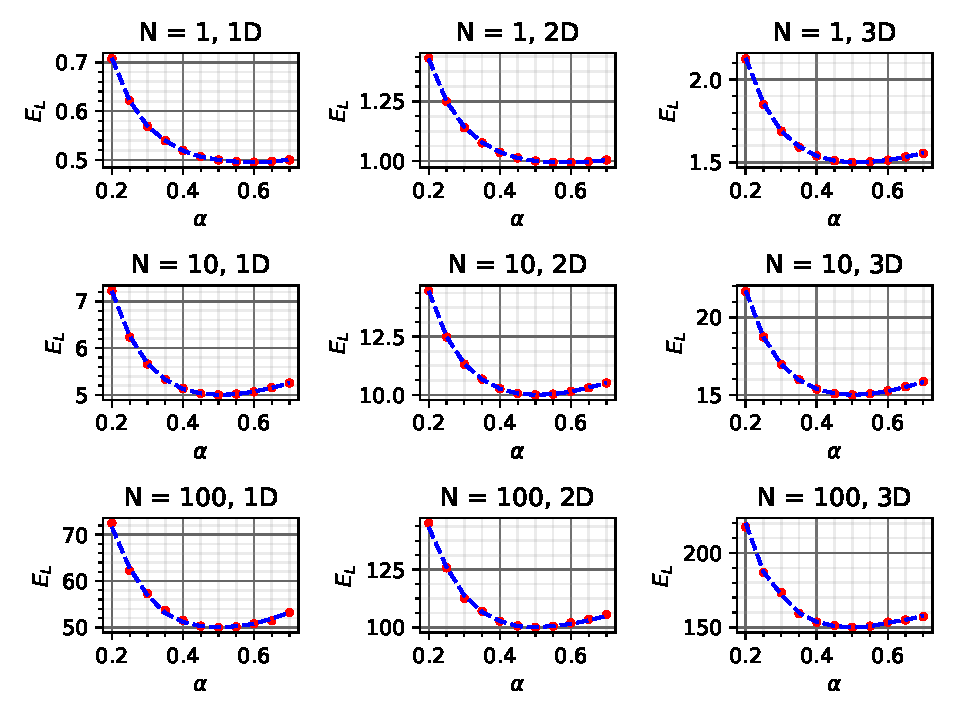
\includegraphics[width=0.5\textwidth]{alpha_1_100_acceptance_ratio_50.pdf}
    \caption{Local energy as a function of $\alpha$ using the standard Metropolis algorithm. This is run for $2^{20}$ number of steps for 1 and 10 particles, whereas 100 particles was only run with $2^{16}$ steps due to the computational time required. The red dots correspond to the analytic calculations, while the blue dashed line corresponds to the numeric calculations.}
    \label{fig:brute_force_spherical_localE}
\end{figure}

\begin{figure}[H]
    \centering
    \includegraphics[width=0.5\textwidth]{blocking_1particle_3d_2e23steps_alpha=0.3_steplength=1_automated.png}
    \caption{Comparison of the biased estimator $\sigma_k^2/n_k$ and $\sigma_b^2$ found through the automated blocking described in ~\ref{subsubsec:blocking}, using a significance level of $\alpha = 0.01$. As can be seen, the plateau is reached at about the sixth iteration, indicating a correlation time of $\tau \sim 2^6$ [You sure?] for a step length of 1. As expected, the behaviour of $\sigma_k^2/n_k$ becomes increasingly erratic for high $k$. This is because the number of blocks are too low to give a good estimate of the sample variance.}
    \label{fig:blocking_behaviour}
\end{figure}

Of course, the number of accepted steps is dependent on the timestep chosen for importance sampling. The relation between the number of accepted steps and the timesteps can be shown in figure~\ref{fig:c_importance_acceptance_ratio_timesteps}, where $\delta t \in [0.1, 1.0]$. Here, we see that the ratio declines as the timesteps increases. Optimally, the timestep $\delta t$ is to be within the range $[0.001, 0.01]$ for stable values of the local energy. We can choose a low timestep, such as $\delta t = 0.001$, but this would require even more computational power as more steps are accepted. Thus, there is a fine line between the desired accuracy of the local energy, and the computational power needed behind the scenes when it comes to importance sampling.


\begin{table}[h!]
 \caption{The computational time required to calculate the local energy. This was run with 3 dimensions, and 1e5 Metropolis steps with a step length of 0.5.}
 \begin{ruledtabular}
    \begin{tabular}{p{0.5cm}p{1.1cm}p{1.1cm}p{1.1cm}p{1.1cm}p{1.1cm}}
    % \toprule
    \multirow{2}{*}{} &
     &
      \multicolumn{2}{l}{Brute Force} &
      \multicolumn{2}{l}{Importance Sampling} \\
    \hline
      N & $\text{E}_{\text{L}}$ & $\text{t}_{\text{anal}}$[\si{\second}] & $\text{t}_{\text{num}}$[\si{\second}]& $\text{t}_{\text{anal}}$[\si{\second}] & $\text{t}_{\text{num}}$[\si{\second}] \\
      \hline
 $1$& 0.5 &  0.1219   &  0.4981   & 0.1633  &  0.6423 \\
 $10$& 5.0 & 0.6938   &   22.2768  & 0.9069    &  29.4808 \\
 $100$& 50.0 &  6.4496  & 2051.1641 &   8.4655    &  2587.9464 \\
 $500$& 250.0 & 32.6107  & $ - $  & 42.3359 & $ - $\\
%    \hline
  \end{tabular}
  \end{ruledtabular}
  \label{tab:c_brute_force_vs_importance_tCPU}
\end{table}

% \begin{table}[h!]
% \caption{Sample measurements of the local energy using the Metropolis-Hastings algorithm, for 1 particle in 3 dimensions. This is run with 1e5 Metropolis steps and a step length of 0.5 and a time step $\delta t = 0.01$.}
% \label{tab:c_importance_sampling_1part_3dim}

% \centering
% \begin{ruledtabular}
% \begin{tabular}{cccccc}
% $\alpha$ & $E_L$  & $\sigma$ & $\sigma_b$ & $A_{ratio}$ & $t_{CPU}[\si{s}]$  \\
% \hline
%           \multicolumn{6}{c}{Analytic}\\
% \hline


% 0.20     & 1.3802 & 0.0009   & 0.0184     & 0.9520      & 1.0247    \\
% 0.25     & 1.2976 & 0.0006   & 0.0141     & 0.9473      & 1.0047    \\
% 0.30     & 1.2969 & 0.0005   & 0.0093     & 0.9431      & 1.0066       \\
% 0.35     & 1.3205 & 0.0003   & 0.0062     & 0.9388      & 0.9951      \\
% 0.40     & 1.3662 & 0.0002   & 0.0022     & 0.9355      & 0.9943       \\
% 0.45     & 1.4284 & 0.0001   & 0.0017     & 0.9317      & 0.9918      \\
% 0.50     & 1.5000 & 0.0000   & 0.0000     & 0.9288      & 0.9922       \\
% 0.55     & 1.5796 & 0.0001   & 0.0013     & 0.9261      & 0.9905       \\
% 0.60     & 1.6655 & 0.0002   & 0.0017     & 0.9230      & 0.9857    \\
% 0.65     & 1.7519 & 0.0002   & 0.0017     & 0.9197      & 0.9779    \\
% 0.70     & 1.8447 & 0.0003   & 0.0042     & 0.9171      & 0.9768   \\
% \hline
%          \multicolumn{6}{c}{Numeric}                                                     \\
% \hline

% 0.20     & 1.3594 & 0.0009   & 0.0174     & 0.9528      & 3.7641    \\
% 0.25     & 1.3035 & 0.0007   & 0.0149     & 0.9478      & 3.7386    \\
% 0.30      & 1.2929 & 0.0005   & 0.0072     & 0.9434      & 3.8651    \\
% 0.35      & 1.3184 & 0.0003   & 0.0070     & 0.9393      & 3.7873    \\
% 0.40     & 1.3662 & 0.0002   & 0.0028     & 0.9351      & 3.7665    \\
% 0.45      & 1.4288 & 0.0001   & 0.0012     & 0.9318      & 3.7455    \\
% 0.50       & 1.5000 & 0.0000   & 0.0000     & 0.9294      & 3.7112    \\
% 0.55     & 1.5789 & 0.0001   & 0.0014     & 0.9255      & 3.7167    \\
% 0.60     & 1.6666 & 0.0002   & 0.0014     & 0.9229      & 3.6921    \\
% 0.65       & 1.7566 & 0.0002   & 0.0029     & 0.9201      & 3.6837    \\
% 0.70     & 1.8482 & 0.0003   & 0.0038     & 0.9173      & 3.6689 \\
% \end{tabular}
% \end{ruledtabular}
% \end{table}


\begin{table}[h!]
\caption{Sample measurements of the local energy using the Metropolis-Hastings algorithm, for 1 particle in 3 dimensions. This is run with 1e5 Metropolis steps and a step length of 1.0 and a time step $\delta t = 0.45$.}
\label{tab:c_importance_sampling_1part_3dim}

\centering
\begin{ruledtabular}
\begin{tabular}{cccccc}
$\alpha$ & $E_L$  & $\sigma$ & $\sigma_b$ & $A_{ratio}$ & $t_{CPU}[\si{s}]$  \\
\hline
          \multicolumn{6}{c}{Analytic}\\
\hline

0.20 &1.4256 &0.0008 &0.0020 &0.7129 &1.5696 \\
0.25 &1.3521 &0.0006 &0.0013 &0.6761 &1.4816 \\
0.30 &1.3371 &0.0004 &0.0009 &0.6415 &1.4160 \\
0.35 &1.3536 &0.0003 &0.0006 &0.6107 &1.3452 \\
0.40 &1.3915 &0.0002 &0.0004 &0.5809 &1.2764 \\
0.45 &1.4415 &0.0001 &0.0002 &0.5520 &1.2402 \\
0.50 &1.5000 &0.0000 &0.0000 &0.5257 &1.2024 \\
0.55 &1.5643 &0.0001 &0.0002 &0.5007 &1.1300 \\
0.60 &1.6326 &0.0002 &0.0003 &0.4761 &1.0480 \\
0.65 &1.7051 &0.0003 &0.0005 &0.4525 &0.9942 \\
0.70 &1.7796 &0.0004 &0.0006 &0.4306 &0.9484 \\ 
\hline
         \multicolumn{6}{c}{Numeric}                                                     \\
\hline

0.20 &1.4231 &0.0008 &0.0020 &0.7126 &5.7639 \\ 
0.25 &1.3536 &0.0006 &0.0014 &0.6770 &5.4619 \\ 
0.30 &1.3364 &0.0004 &0.0009 &0.6418 &5.1868 \\ 
0.35 &1.3541 &0.0003 &0.0006 &0.6117 &4.9487 \\ 
0.40 &1.3916 &0.0002 &0.0004 &0.5808 &4.6998 \\ 
0.45 &1.4414 &0.0001 &0.0002 &0.5531 &4.4726 \\ 
0.50 &1.5000 &0.0000 &0.0000 &0.5258 &4.2706 \\ 
0.55 &1.5644 &0.0001 &0.0002 &0.4999 &4.0544 \\ 
0.60 &1.6323 &0.0002 &0.0003 &0.4766 &3.8601 \\ 
0.65 &1.7048 &0.0003 &0.0005 &0.4528 &3.6759 \\ 
0.70 &1.7787 &0.0004 &0.0006 &0.4307 &3.4941
\end{tabular}
\end{ruledtabular}
\end{table}

\begin{figure}[h!]
    \centering
    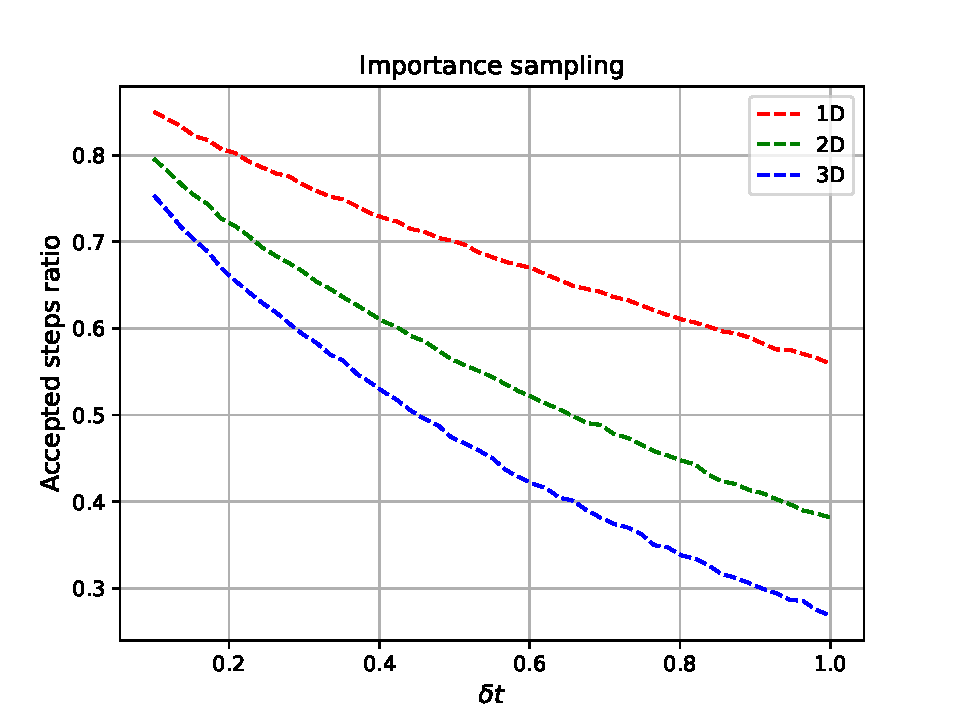
\includegraphics[width=0.5\textwidth]{accepted_ratio_vs_timesteps_nPart1_MC100000.pdf}
    \caption{The ratio of accepted steps compared to the timestep $\delta t\in [0.1, 1.0]$ as computed by the Metropolis-Hasting algorithm. This was run with 1 particle, in $d = 1, 2, 3$ dimensions, with $2^{19}$ Metropolis steps.}
    \label{fig:c_importance_acceptance_ratio_timesteps}
\end{figure}

\subsection{Interacting elliptical system}
Now, we turn to the system in which we include the repulsive potential through the Jastrow factor in eq.~\eqref{eq:trial_wavefunction_total}. Here, we set $\beta = 2.82843$ and $a=0.0043$, thus allowing us to look at an elliptical, interacting boson system. From here on out, we will mainly use the Standard Metropolis algorithm.

\subsubsection{Local energy}
The local energy for an interacting elliptical system in 3 dimensions for $N=10$, 50 and 100 particles can be seen in table~\ref{tab:e_brute_force_localE_stepLength_1.0}. Here, due to the computational power required to perform these calculations we had to scale down the number of Metropolis steps run for the $N$ particles. For $N=10$ and 50 we ran $2^{17}$ Metropolis steps, whereas for $N=100$ we ran $2^{16}$ Metropolis steps. We only start sampling the energy after about $5\%$ of the Metropolis steps have been run, to allow for the calibration of the energy.
As one can see, due to the lower number of Metropolis steps, the error will increase as the total sample size decreases.


\subsubsection{Optimal parameter}
Using the method of gradient descent we can try to find the optimal variational parameter $\alpha$ which will lead to a minimal value of the local energy. This can be seen in figure~\ref{fig:f_gradient_descent}, where we find the local energy using $2^{17}$ steps over 100 iterations. This is done using a learning rate of $\gamma = 0.1$, and test values of $\alpha \in [0.1, 0.9]$.
Taking the mean of $\alpha$ at the 100'th iteration for each test value of $\alpha$, we get that the optimal parameter is $$\alpha = 0.514232 \pm 0.013922.$$
\begin{figure}[h!]
    \centering
    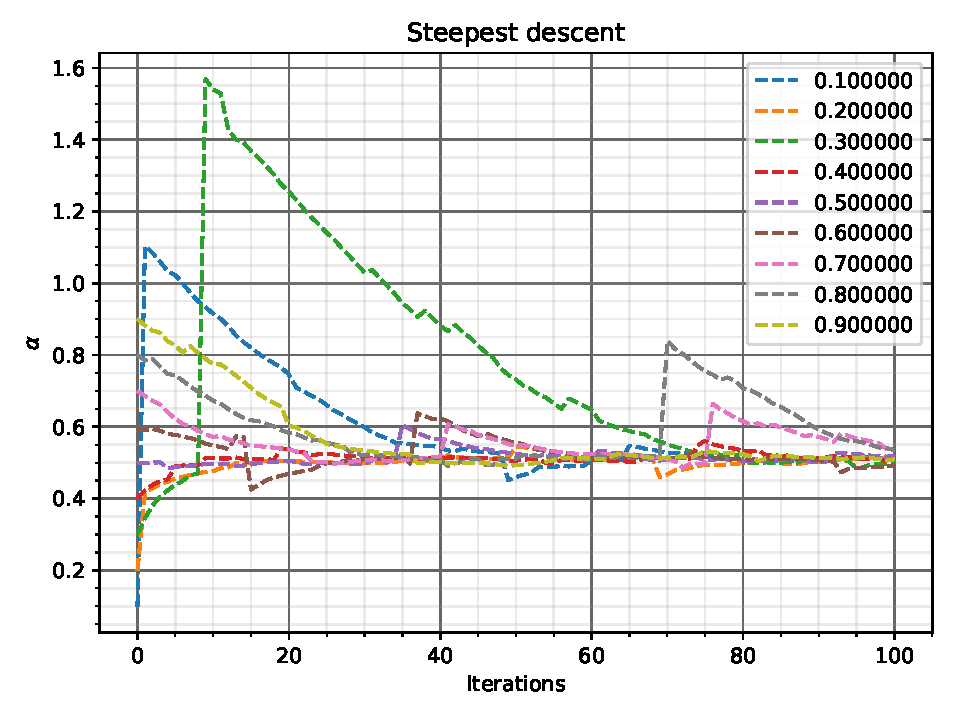
\includegraphics[width=0.5\textwidth]{steepest_descent_nSteps_131072.pdf}
    \caption{Gradient descent using $2^{17}$ Metropolis steps and a learning rate $\gamma_k = 0.1$.}
    \label{fig:f_gradient_descent}
\end{figure}

\subsubsection{One-body density}
The one-body densities are shown in figure~\ref{fig:g_onebody_density}, where we have plotted the density for the ellipsoidal system with and without the Jastrow factor as well as the spherical non-interacting system. As in \cite{vortex} and \cite{trapped}, we have set $a/a_{ho} = 0.0043$ and $\beta = \sqrt{8}$. The figure illustrates that the effect of including the Jastrow factor, viz. interaction, is to spread out the particles. This is because the hard-core radius prevents the particles from stacking up on each other. This effect would be more pronounced for a larger number of particles. 

Note that the one-body density for the spherical wavefunction is smaller than that of the elliptical wavefunction. This is to be expected, as $\Delta V$ increases by a factor of $\sqrt{\beta}$ when integrating over spherical shells compared to elliptical ones. From equation \eqref{eq:29}, the elliptical one-body density should therefore be a factor of $\sqrt{\beta}$ greater than the spherical. A rough estimate from figure \ref{fig:g_onebody_density} reveals this factor to be $1.666 \approx 1.682 = \sqrt{\beta}$.

\begin{table}[H]

\caption{Local energy as a function of $\alpha$ when running the brute force algorithm for $N = 10$, 50 and 100 particles in 3 dimensions. This is done with $2^{17}$ steps for $N=10, 50$, whereas the computation for $N=100$ is done with $2^{16}$ steps. All is run with a step length 1.0.}
\label{tab:e_brute_force_localE_stepLength_1.0}
% \makebox[0.45 \textwidth][c]{       %centering table
% \resizebox{0.45 \textwidth}{!}{   %resize table
\centering
\resizebox{0.5\textwidth}{!}{%
\begin{ruledtabular}
\begin{tabular}{ccccc}

$\alpha$ & $E_L$   & $\sigma$ & $\sigma_b$ & $A_{ratio}$ \\
\hline
    \multicolumn{5}{c}{10 particles} \\              
\hline
0.20 &36.3429 &0.1635 &0.2623 &0.6489 \\
0.25 &31.0444 &0.0860 &0.0625 &0.6150 \\
0.30 &28.5313 &0.0374 &0.0541 &0.5851 \\
0.35 &27.0695 &0.0991 &0.0242 &0.5588 \\
0.40 &30.9139 &1.9405 &0.5084 &0.5342 \\
0.45 &26.4922 &0.1349 &0.1914 &0.5114 \\
0.50 &30.0830 &1.1763 &0.0470 &0.4914 \\
0.55 &28.8557 &0.8074 &0.3922 &0.4732 \\
0.60 &27.5154 &0.1505 &0.2982 &0.4554 \\
0.65 &27.2751 &0.3708 &0.1506 &0.4395 \\
0.70 &28.5333 &0.1853 &0.0816 &0.4241 \\
\hline
\multicolumn{5}{c}{50 particles}               \\
\hline
0.20     & 190.3719 & 0.1971   & 0.457067    & 0.5454       \\
0.25     & 167.2134 & 0.2417   & 0.605498    & 0.5454
0.30     & 166.5803 & 0.8381   & 2.10527     & 0.5114    \\
0.35     & 155.6323 & 0.4971   & 1.30742     & 0.4831   \\
0.40     & 182.5975 & 2.8327   & 4.74049     & 0.4569      \\
0.45     & 158.9000 & 1.4974   & 1.52235     & 0.4335           \\
0.50     &  163.9296 & 3.7315  & 2.27611     & 0.4106     \\
0.55     & 166.6583 & 1.3770   & 2.64776     & 0.3915     \\
0.60     & 167.3481 & 0.8089   & 6.65364     & 0.3744    \\
0.65     & 234.4480 & 4.1277   & 12.0293     & 0.3597        \\
0.70     & 237.2478 & 8.8231   & 3.11682     & 0.3440          \\
\hline
\multicolumn{5}{c}{100 particles}               \\
\hline

0.20     & 444.8302 & 3.6103   & 11.057     & 0.5713      \\
0.25     & 353.9400 & 0.4392   & 1.08801    & 0.5377      \\
0.30     & 361.6295 & 1.7793   & 5.68786    & 0.5084      \\
0.35     & 350.0379 & 3.2279   & 4.18892    & 0.4792      \\
0.40     & 484.9373 & 10.3091  & 38.1289    & 0.4542      \\
0.45     & 370.9348 & 5.8136   & 6.13453    & 0.4317      \\
0.50     & 417.5323 & 6.0516   & 4.80259    & 0.4138      \\
0.55     & 367.7318 & 1.7960   & 9.79242    & 0.3913      \\
0.60     & 413.8120 & 2.2802   & 6.65364    & 0.3754      \\
0.65     & 527.4375 & 4.3581   & 12.0293    & 0.3587      \\
0.70     & 411.8401 & 2.9253   & 3.11682    & 0.3450     \\
\end{tabular}
\end{ruledtabular}
}
\end{table}

\begin{figure}[H]
    \centering
    \includegraphics[width=0.45\textwidth]{onebodydensity_steplength0.1_nbins500_nsteps1e7.png}
    \caption{One-body density vs. radial distance in units of $a_{ho}$. This was run with 20 particles in 3 dimensions, with a steplength of 0.1 and 1e7 number of Metropolis steps.}
    \label{fig:g_onebody_density}
\end{figure}




%----------------------------------------------------------------------
%   DISCUSSION SECTION
%----------------------------------------------------------------------
\section{Discussion}
\subsection{Non-interacting spherical system}
\subsubsection{Standard Metropolis}
From table~\ref{tab:b_bruteforce_1part_3dim} we see that the brute force method allows us to calculate the local energy with a small margin for error. The analytic method requires less computational power as it does not require multiple evaluations of the wavefunction at different time steps when computing the double derivative required for the kinetic energy. As for the numeric version, the double derivative does require this evaluation at different time steps.

In figure~\ref{fig:brute_force_spherical_localE} we see that the analytic and numeric approximations to the local energy as a function of $\alpha$ agrees quite well, in all dimensions. The local energy reaches a minimum around $\alpha = 0.5$ as expected.

\subsubsection{Adding importance sampling}
When adding importance sampling, as can be seen in table~\ref{tab:c_importance_sampling_1part_3dim}, we do not assume a symmetric distribution. Here, the biased error $\sigma$ appears smaller than that of the brute force method, which is due to the acceptance ratio being higher in this case. We can also see that the blocking error for importance is somewhat smaller for some of the parameters of $\alpha$.. This is due to the fact that the autocorrelation time $\tau$ increases along with the accepted number of steps.

%For the exact same parameters, the biased sample variance is higher for brute force compared to importance sampling. This is shown in  figure (...). This is for the sp

The computational time required for importance sampling is longer than that of brute force, as can be seen in table~\ref{tab:c_brute_force_vs_importance_tCPU}. This is due to the additional computational power required in calculating the quantum force, as expressed in eq.~\eqref{eq:drift_force_non-interacting}.

\subsection{Interacting elliptical system}
\subsubsection{Local energy}
The local energy when including interaction between the bosons in an elliptical system can be seen in table~\ref{tab:e_brute_force_localE_stepLength_1.0}. Here, $E_L$ seems to fluctuate a bit, and reaches a minimum around $\alpha = 0.45$. From the blocking error we also see that there is a bit uncertainty around the numbers produced. This can also be due to the number of Metropolis steps chosen to produce the energies. We made an attempt at keeping the number of accepted steps $A_{ratio}\sim 0.5$ in order to minimize the autocorrelation time, giving us a more realistic blocking error. The reasoning is explained a bit further down in the section 'Extra Remarks'. As the number of particles also increases, the error increases as well.

\subsubsection{Optimal parameter}
From the use of gradient descent we find that the most optimal value of $\alpha$ for an interacting, elliptical system is $\alpha = 0.514232\pm 0.013922$. Figure~\ref{fig:f_gradient_descent} shows the learning curve of approaching $\alpha$, when starting out with an initial 'guess' value. We could have chosen a smaller learning rate, which would hopefully converge to a more precise value of $\alpha$, but this would then have required more iterations. Another thing to be aware of is the sudden spikes in $\alpha$, especially for $\alpha_0 = 0.1, 0.3$ and 0.8, although they converge back to $\alpha \sim 0.51$.

\subsubsection{One-body density}
The one-body density is found by estimating the integral in eq. \eqref{eq:onebody_density_integral} by use of Monte Carlo integration. As explained in section~\ref{subsubsec:one_body}, we sum the one-body densities of all the particles rather than calculating the one-body density of an arbitrary particle in the ensemble. This is to save CPU cycles. To get a reasonably smooth plot, we needed 1e7 Monte Carlo steps for 20 particles. Sampling the position of every particle at each step is a lot cheaper than increasing the number of steps by a factor of $20$ and only sampling the position of one particle each time.

Ideally we would like to plot the one-body density for 100 particles to see a more pronounced spread for the interacting case compared to the non-interacting. The drastic increase in run-time is what prevented us from doing so. Future improvements would include optimizing our code so as to make this possible. 

Our initial plots of the one-body density were suboptimal due to the way we estimated $\Delta V$. For a discussion on this, see Appendix G.


%----------------------------------------------------------------------
%   FURTHER DEVELOPMENTS SECTION
%----------------------------------------------------------------------
\section{Extra remarks}\label{sec:extra_remarks}
As can be seen from table~\ref{tab:e_brute_force_localE_stepLength_1.0} there is a noticeable difference between the error as calculated by the Monte Carlo runs and the blocking error. This is due to the autocorrelation time $\tau$. If we had adjusted the step length in such a way that the number of accepted steps increased, then the time between a sample and the next uncorrelated sample would increase, thus resulting in a higher blocking error. This is illustrated in table~\ref{tab:e_brute_force_localE_stepLength_0.1} below, where each measurement of the local energy has been run using a step length of 0.1. Here, we see that the blocking error drastically increases, along with the number of particles, compared to the blocking error from table~\ref{tab:e_brute_force_localE_stepLength_1.0}.

%----------------------------------------------------------------------
%   CONCLUSION SECTION
%----------------------------------------------------------------------
\section{Conclusion}
Throughout this report we have attempted to find the local energy of both a non-interacting as well as an interacting boson system. This has been done in all 3 dimensions for $N = 1, 10, 50, 100$ and 500 particles. We started out with a non-interacting, spherical boson system using the Standard Metropolis algorithm, which allowed us to find an approximation to the minima of the local energy at $\alpha = 0.5$. 
Furthermore, we added importance sampling to the same system and observed the effects it had on the blocking error along with some additional computational time compared to that of the brute force method.

 We have also examined how the Jastrow factor, i.e. an interacting system, affects the local energy when dealing with an elliptical potential. This was done using the brute force method. We also studied how to find the optimal variational parameter $\alpha$ leading to a minima of the local energy, although one must be aware that the method used, that is gradient descent, has a tendency to converge to a local minima of a system, and not necessarily the global minima.
 
 Finally, we studied the one-body densities in the ellipsoidal system both with and without the Jastrow factor. Here, we found that the effects of including the Jastrow factor leads to a larger spread between the bosons and thus a lower density compared to that of a non-interacting system.

\begin{table}[H]

\caption{Local energy as a function of $\alpha$ when running the brute force algorithm for $N = 10$, 50 and 100 particles in 3 dimensions. This is done with $2^{17}$ steps for $N=10, 50$, whereas the computation for $N=100$ is done with $2^{16}$ steps. All is run with a step length 0.1.}
\label{tab:e_brute_force_localE_stepLength_0.1}
% \makebox[0.45 \textwidth][c]{       %centering table
% \resizebox{0.45 \textwidth}{!}{   %resize table
\centering
\resizebox{0.5\textwidth}{!}{%
\begin{ruledtabular}
\begin{tabular}{ccccc}

$\alpha$ & $E_L$   & $\sigma$ & $\sigma_b$ & $A_{ratio}$ \\
\hline
    \multicolumn{5}{c}{10 particles} \\              
\hline
0.20     & 34.0713 & 0.0611   & 1.6308     & 0.9281        \\
0.25     & 31.5360 & 0.0342   & 0.7784     & 0.9212       \\
0.30     & 28.2917 & 0.0539   & 0.8228     & 0.9189         \\
0.35     & 25.8278 & 0.0823   & 0.7285     & 0.9159        \\
0.40     & 25.9493 & 0.5688   & 1.0597     & 0.9104         \\
0.45     & 26.9736 & 0.1466   & 1.2192     & 0.9060         \\
0.50     & 27.1611 & 0.1133   & 2.1561     & 0.9056     \\
0.55     & 24.7051 & 0.8227   & 4.2643     & 0.8992        \\
0.60     & 30.1142 & 0.2282   & 10.5249    & 0.8982    \\
0.65     & 27.3815 & 0.4034   & 1.8682     & 0.8938       \\
0.70     & 28.3706 & 0.2960   & 2.6699     & 0.8908      \\
\hline
\multicolumn{5}{c}{50 particles}               \\
\hline
0.20     & 190.1579 & 3.4246   & 15.9905    & 0.9306     \\
0.25     & 194.2594 & 2.3330   & 4.0890     & 0.9236       \\
0.30     & 128.8150 & 5.3416   & 5.0189     & 0.9196      \\
0.35     & 180.0029 & 2.5183   & 11.7675    & 0.9178    \\
0.40     & 132.1552 & 1.5432   & 9.5690     & 0.9112        \\
0.45     & 200.1127 & 1.9996   & 34.1202    & 0.9068     \\
0.50     & 182.7901 & 0.8094   & 19.4530    & 0.9035       \\
0.55     & 154.4427 & 1.0658   & 15.5231    & 0.9028    \\
0.60     & 161.1288 & 0.5748   & 24.0146    & 0.9015        \\
0.65     & 253.8886 & 2.2427   & 29.1721    & 0.8947       \\
0.70     & 207.7466 & 1.4643   & 113.9832   & 0.8939       \\
\hline
\multicolumn{5}{c}{100 particles}               \\
\hline

0.20     & 624.8332 & 16.4875  & 504.4450   & 0.9051      \\
0.25     & 631.0877 & 21.3615  & 9.6819     & 0.8955      \\
0.30     & 346.0408 & 2.1510   & 11.2545    & 0.8898      \\
0.35     & 466.0410 & 17.7181  & 46.5227    & 0.8852      \\
0.40     & 390.7578 & 1.1315   & 25.2673    & 0.8816      \\
0.45     & 326.9681 & 7.6810   & 60.7939    & 0.8774      \\
0.50     & 802.4169 & 17.0915  & 93.5271    & 0.8782      \\
0.55     & 495.5016 & 7.2860   & 9.1320     & 0.8753      \\
0.60     & 410.5282 & 1.7056   & 52.0087    & 0.8719      \\
0.65     & 969.0100 & 10.1001  & 41.0221    & 0.8674      \\
0.70     & 787.3473 & 35.4289  & 152.2204   & 0.8661    \\
\end{tabular}
\end{ruledtabular}
}
\end{table}

% \begin{table}
%     \caption{Importance sampled simulations of $N=10$ particles in
%     $d=3$ dimensions. Average acceptance ratios and standard
%     deviations for eleven values of $\alpha \in [0.3, 0.7]$.}
%     \centering
%         \begin{ruledtabular}
%             \begin{tabular}{cccc}
%                 $\delta t$ & $\bar{\sigma}_b$ & $\bar{A}$
%                 & $\expval{E}\left(\alpha = 1/2\right)$ \\
%                 \hline
%                 $2^{+3}$ & 0.09363 & 0.005 & 15.000 \\
%                 $2^{+2}$ & 0.01549  & 0.041 & 15.000 \\
%                 $2^{+1}$ & 0.00706 & 0.216 & 15.000 \\
%                 $2^{\ 0}$ & 0.00675 & 0.510 & 15.000 \\
%                 $2^{-1}$ & 0.00932 & 0.738 & 15.000 \\
%                 $2^{-2}$ & 0.01578 & 0.866 & 15.000 \\
%                 $2^{-3}$ & 0.02723 & 0.933 & 15.000 \\
%                 $2^{-4}$ & 0.05016 & 0.966 & 15.000 \\
%                 $2^{-5}$ & 0.08474 & 0.983 & 15.000 \\
%                 $2^{-6}$ & 0.11555 & 0.992 & 15.000 \\
%                 $2^{-7}$ & 0.17070 & 0.996 & 15.000 \\
%             \end{tabular}
%         \end{ruledtabular}
%         \label{tab:imp_time_step}
% \end{table}


\printbibliography

%%%%%%%%%%%%%%%%%%%%%%%%%%%%%%%%%%%%%%%%%%%%%%%%%%%%%%%%%%%%%%%%%%%%%%%%%%%%%%%%%%%%%%%%%%%%%%%%%%%%%
\newpage
\begin{appendices}

\section{Trial wavefunction}
The trial wavefunction is given by
\begin{align}\label{trial_wavefunction}
    \Psi_T(\boldsymbol{r}) &= \Psi_T(\boldsymbol{r}_1,\boldsymbol{r}_2,...,\boldsymbol{r}_N,\alpha,\beta) \\
    &= \left[\prod_i g(\alpha,\beta,\boldsymbol{r}_i)\right] \left[\prod_{j<k} f(a,|\boldsymbol{r}_j - \boldsymbol{r}_k|)\right] \nonumber
\end{align}
Where
\begin{equation}\label{eq:2}
    f(a,|\boldsymbol{r}_i - \boldsymbol{r}_j|) =
    \begin{cases}
      0 & |\boldsymbol{r}_i - \boldsymbol{r}_j|\leq a \\
     \left(1-\frac{a}{|\boldsymbol{r}_i - \boldsymbol{r}_j|}\right) & |\boldsymbol{r}_i - \boldsymbol{r}_j| > a\\
    \end{cases} 
\end{equation}
Is the correlation wavefunction and 
\begin{equation}
    g(\alpha, \beta, \boldsymbol{r}_i) =  \exp[-\alpha(x_i^2 + y_i^2 + \beta z_i^2)]
\end{equation}
Where $\alpha$ and $\beta$ are variational parameters. $\beta = 1$ for spherical traps  and for non-interacting bosons ($a=0$) we have $\alpha = 1/2a_{ho}^2$ 
\newline
\section{Local Energy}\label{appendix:local_energy}
We want to find the local energy  
\begin{equation}\label{local_energy}
   E_L(\boldsymbol{r}) =  \frac{1}{\Psi_T(\boldsymbol{r})} H \Psi_T(\boldsymbol{r})
\end{equation}
For the harmonic oscillator potential in one, two and three dimensions with
\begin{align*}
    a&=0 \quad \text{Non-interacting potential} \\
    \beta& = 1 \quad \text{Spherically symmetric potential}
\end{align*}
For $N$ particles. The external potential in this case is given by 
\begin{equation}
    V_{ext} =
    \begin{cases}
      \frac{1}{2}m \omega_{ho}^2 x^2 &  1\text{D}\\
     \frac{1}{2}m \omega_{ho}^2\left( x^2 +  y^2 \right) & 2\text{D}\\
     \frac{1}{2}m \omega_{ho}^2\left(x^2 +  y^2 +z^2 \right) & 3\text{D}
    \end{cases} 
\end{equation}
And the Hamiltonian is 
\begin{equation}
    H = \sum_i^N \left(\frac{-\hbar^2}{2m} \nabla_i^2 + V_{ext}(\boldsymbol{r}_i)\right)
\end{equation}
Inserting $a=0$ into \eqref{eq:2} gives $f(a,|\boldsymbol{r}_i - \boldsymbol{r}_j|) =1$ and so
\begin{equation}
    \Psi_T = \prod_i g(\alpha,\beta,\boldsymbol{r}_j) = \prod_j \exp\left[ -\alpha \left(x_j^2 + y_j^2 + z_j^2\right)\right]
\end{equation}
Next, we calculate the Laplacian of the trial wavefunction. Differentiating only with respect to $x$ gives
\begin{align*}
    \frac{\partial^2}{\partial x_i^2} \Psi_T &= \frac{\partial}{\partial x_i} \left(-2\alpha x_i \prod_j \exp\left[ -\alpha \left(x_j^2 + y_j^2 + z_j^2\right)\right] \right)\\
    &= 2\alpha \left(2\alpha x_i^2 -1\right) \prod_j \exp\left[ -\alpha \left(x_j^2 + y_j^2 + z_j^2\right)\right]
\end{align*}
Repeating the same calculation for the $y$ and $z$ coordinates yields
\begin{equation}
\nabla_i^2 \Psi_T = 2\alpha \left(2\alpha \boldsymbol{r}_i^2 -3\right) \Psi_T
\end{equation}
This can be generalized for a system of dimension $d\in [1,2,3]$ to
\begin{equation}
\nabla_i^2 \Psi_T = 2\alpha \left(2\alpha \boldsymbol{r}_i^2 -d\right) \Psi_T
\end{equation}
Inserting this into eq. \eqref{local_energy} gives 
\begin{equation}\label{local_energy_applied}
    E_L = \frac{1}{\Psi_T} \sum_i^N \left[\frac{-\hbar^2}{2m} 2\alpha(2\alpha \boldsymbol{r}_i^2 - d) \Psi_T + \frac{1}{2}m \omega_{ho}^2 \boldsymbol{r}_i^2 \Psi_T\right]
\end{equation}
Since we are dealing with non-interacting bosons, $\alpha = 1/2 a_{ho}^2 = \frac{m\omega_{ho}}{2\hbar}$. Inserting this into eq. \eqref{local_energy_applied} makes the first and last terms cancel, and we are left with
\begin{equation}
    E_L = \frac{d}{2} \hbar \omega_{ho} N
\end{equation}
Where $d\in [1,2,3]$ is the dimension of our system and $N$ the number of particles. 
The drift force is given by 
\begin{align}
    F &= \frac{2\nabla \Psi_T}{\Psi_T}\\
    &= \frac{2}{\Psi_T}\nabla_i\prod_j \exp[-\alpha(x_j^2+y_j^2+z_j^2)] \\ 
    &= \frac{2}{\Psi_T} \left(-2\alpha (x_i \hat{i}+ y_i \hat{j} + z_i \hat{k})\right) \Psi_T \\
\end{align}
Or in general 
\begin{equation}
    F =-4\alpha \boldsymbol{r}_i
\end{equation}
Where $\boldsymbol{r}_i = x_i \hat{i} + y_i \hat{j}$ in 2D and $\boldsymbol{r}_i = x_i \hat{i}$ in 1D.
\section{First derivative}
The trial wavefunction \cite{project1}
\begin{align}
    \Psi_T(\boldsymbol{r}) &= \Psi_T(\boldsymbol{r}_1,\boldsymbol{r}_2,...,\boldsymbol{r}_N,\alpha,\beta) \\
    &= \left[\prod_i g(\alpha,\beta,\boldsymbol{r}_i)\right] \left[\prod_{j<k} f(a,|\boldsymbol{r}_j - \boldsymbol{r}_k|)\right]
\end{align}
Can be rewritten as 
\begin{equation}
    \Psi_T(\boldsymbol{r}) = \left[\prod_i \phi(\boldsymbol{r}_i)\right] \exp \left(\sum_{j<k} u(r_{jk})\right)
\end{equation}
By defining 
\begin{align*}
     \phi(\boldsymbol{r}_i) \equiv & g(\alpha, \beta, \boldsymbol{r}_i) =  \exp[-\alpha(x_i^2 + y_i^2 + z_i^2)]  \\
    r_{ij} \equiv& |\boldsymbol{r}_i - \boldsymbol{r}_j|
\end{align*}
and 
\begin{equation}
    f(r_{ij}) = \exp \left(\sum_{i<j} u(r_{ij})\right)
\end{equation}
Where $u(r_{ij}) = \ln{f(r_{ij})}$. 
The first derivative for particle $k$ is then 
\begin{align}
    \nabla_k \Psi_T(\boldsymbol{r}) &= \left[\nabla_k \prod_i \phi(\boldsymbol{r}_i)\right]\exp\left(\sum_{j<k} u(r_{jk})\right) \nonumber \\ 
    &+ \left[\prod_i \phi(\boldsymbol{r}_i)\right]\nabla_k \exp\left(\sum_{j<k} u(r_{jk})\right) 
\end{align}
Where the derivative of the exponential is
\begin{align}\label{exponential_deriv}
    \nabla_k \exp\left(\sum_{j<m} u(r_{jm})\right) = \exp\left(\sum_{j<m} u(r_{jm})\right)  \sum_{j < m} \nabla_k u(r_{jm}) 
\end{align}
And the sum 
\begin{align}
    \sum_{j<m} u(r_{jm}) =\sum_{j=1}\sum_{m=j+1} u(r_{jm})& \\
    = \left[u(r_{12})+u(r_{13})+...+u(r_{1N})\right]& \nonumber \\
    + \left[u(r_{23})+...+u(r_{2N})\right]& \nonumber \\
     \ddots \qquad \qquad \vdots \qquad& \nonumber \\
    +\left[u(r_{N-1,N})\right] \nonumber
\end{align}
Ensures that every particle couples once to every other particle except itself. We see that the order in which they couple is not consistent, but because $r_{jm}$ is symmetric under interchange of indices, we get 
\begin{equation}
    \sum_{j<m }\nabla_k  u(r_{jm}) = \sum_{l\neq k } \nabla_k u(r_{kl})
\end{equation}
The derivative of the product is simply 
\begin{equation}
    \nabla_k \prod_{i}\phi(\boldsymbol{r}_i) = \nabla_k \phi(\boldsymbol{r}_k) \prod_{i \neq k} \phi(\boldsymbol{r}_i)
\end{equation}
And so the first derivative of the trial wavefunction is
\begin{align}
    \nabla_k \Psi_T(\boldsymbol{r}) =& \nabla_k \phi(\boldsymbol{r_k}) \left[\prod_{i \neq k} \phi(\boldsymbol{r}_i)\right] \exp\left(\sum_{j<m} u(r_{jm})\right) \\
    &+ \left[\prod_i \phi(\boldsymbol{r}_i)\right]\exp \left(\sum_{j<m} u(r_{jm})\right) \sum_{l\neq k} \nabla_k u(r_{kl}) \nonumber
\end{align}



\section{Second derivative}

\begin{align}
   & \frac{1}{\Psi_T(\vec r)} \nabla^{2}_{k} \Psi_{T}(\boldsymbol{r}) = \frac{1}{\left[\prod_{i}\phi(\boldsymbol{r}_i)\right]\exp\left({\sum^{}_{i<j} u(r_{ij})}\right)} \Bigg\{ \\ &\nabla^{2}_{k}\phi(\boldsymbol{r}_k)\left[ \prod_{i \neq k} \phi(\boldsymbol{r}_i) \right] \exp\left(\sum_{j<m} u(r_{jm}) \right) \tag{i}\label{eq:i} \\
    &+\nabla_{k}\phi(\boldsymbol{r}_k)\left[ \prod_{i \neq k} \phi(\boldsymbol{r}_i) \right] \nabla_{k}\exp\left(\sum_{j<m} u(r_{jm})\right) \tag{ii}\label{eq:ii}\\
    &+\left[\nabla_k \prod_{i} \phi(\boldsymbol{r}_i)\right]  \exp\left(\sum_{j<m} u(r_{jm})\right) \sum_{j\neq k} \nabla_{k} 
    u(r_{kj})  \tag{iii}\label{eq:iii}
    \\\
    &+\left[\prod_{i} \phi(\boldsymbol{r}_i)\right] \left[ \nabla_k \exp\left(\sum_{j<m} u(r_{jm})\right) \right] \sum_{j\neq k} \nabla_{k} u(r_{kj})  \tag{iv}\label{eq:iv}\\
    &+
    \left[\prod_{i} \phi(\boldsymbol{r}_i)\right] \exp\left(\sum_{j<m} u(r_{jm})\right) \nabla_k \sum_{j\neq k} \nabla_{k} u(r_{kj}) \Bigg\} \Bigg. \tag{v}\label{eq:v}
\end{align}
Using 
\begin{equation*}
    \frac{\prod_{i \neq k} \phi(\boldsymbol{r}_i)}{\prod_i \phi(\boldsymbol{r}_i)} = \frac{1}{\phi(\boldsymbol{r}_k)}
\end{equation*}
And eq.\eqref{exponential_deriv}, the first three terms can be contracted to yield
\begin{equation}\label{i+ii+iii}
    \eqref{eq:i}+\eqref{eq:ii} + \eqref{eq:iii} = \frac{\nabla_i^2 \phi(\boldsymbol{r}_k)}{\phi(\boldsymbol{r}_k)} + 2\frac{\nabla_k \phi(\boldsymbol{r}_k)}{\phi(\boldsymbol{r}_k)} \sum_{j\neq k} \nabla_k u(r_{jm})
\end{equation}
$\nabla_k u(r_{jm})$ can be calculated by use of the chain rule
\begin{align}\label{grad_k_u}
    \nabla_k u(r_{kj}) =& \left( \frac{\partial}{\partial x} \hat{i} + \frac{\partial}{\partial y} \hat{j} + \frac{\partial}{\partial z} \hat{k} \right) u(r_{kj}) \\
    = &\left( \frac{\partial r_{kj}}{\partial x} \hat{i} + \frac{\partial r_{kj}}{\partial y} \hat{j} + \frac{\partial r_{kj}}{\partial z} \hat{k} \right) \frac{\partial u(r_{kj})}{\partial r_{kj}} \nonumber
\end{align}
 Where
\begin{align}
    \frac{\partial r_{kj}}{\partial x} \hat{i} =& \frac{\partial}{\partial x} \left| \boldsymbol{r}_k - \boldsymbol{r}_j \right|\hat{i} \\
    =& \frac{\partial}{\partial x} \sqrt{(x_k-x_j)^2+(y_k-y_j)^2+(z_k-z_j)^2} \hat{i} \nonumber  \\
    =& \frac{(x_k-x_j)}{r_{kj}} \hat{i} \nonumber
\end{align}
And similarly for the y and z derivatives. Equation \eqref{grad_k_u} therefore becomes 
\begin{equation*}
    \nabla_k u(r_{kj}) = \frac{\boldsymbol{r}_k-\boldsymbol{r}_j}{r_{kj}} u'(r_{kj})
\end{equation*}
Where $u'(r_{kj}) \equiv  \frac{\partial u(r_{kj})}{r_{kj}}$.
Inserting this back into eq.\eqref{i+ii+iii} yields 
\begin{equation}
     \eqref{eq:i}+\eqref{eq:ii} + \eqref{eq:iii} = \frac{\nabla_i^2 \phi(\boldsymbol{r}_k)}{\phi(\boldsymbol{r}_k)} + 2\frac{\nabla_k \phi(\boldsymbol{r}_k)}{\phi(\boldsymbol{r}_k)} \sum_{j\neq k} \frac{\boldsymbol{r}_k-\boldsymbol{r}_j}{r_{kj}} u'(r_{kj})
\end{equation}
After differentiating the exponent, the fourth term reduces to 
\begin{align}
    \eqref{eq:iv} &= \sum_{i\neq k} \nabla_k u(r_{ki}) \sum_{j\neq k} \nabla_k u(r_{kj}) \nonumber\\
    &= \sum_{i\neq k} \sum_{j\neq k} \left(\nabla_k u(r_{ki})\right) \left(\nabla_k u(r_{kj})\right)\nonumber \\
    &= \sum_{i\neq k} \sum_{j \neq k} \frac{\left(\boldsymbol{r}_k - \boldsymbol{r}_i\right)\left(\boldsymbol{r}_k - \boldsymbol{r}_j\right)}{r_{ki} r_{kj}} u'(r_{ki}) u'(r_{kj})
\end{align}
After cancelling terms in the numerator and denominator of the fifth term, one is left with 
\begin{align}\label{v}
    \eqref{eq:v} &= \nabla_k \sum_{j\neq k} \nabla_k u(r_{kj}) = \sum_{j \neq k} \nabla_k \left[\frac{\boldsymbol{r}_k - \boldsymbol{r}_j}{r_{kj}} u'(r_{kj})\right] \nonumber \\
    &= \underbrace{\sum_{j\neq k}   \left[\nabla_k \frac{\boldsymbol{r}_k - \boldsymbol{r}_j}{r_{kj}}\right]u'(r_{kj})}_{\big{i'}} +\underbrace{\frac{\boldsymbol{r}_k - \boldsymbol{r}_j}{r_{kj}}\nabla_k u'(r_{kj})}_{\big{ii'}} 
\end{align}
Let's calculate the first term, $\big{i'}$. Using the product rule
gives
\begin{align}
    \nabla_k \frac{\boldsymbol{r}_k - \boldsymbol{r}_j}{r_{kj}} = \frac{\left[\nabla_k (\boldsymbol{r}_k - \boldsymbol{r}_j) \right]r_{kj} - (\boldsymbol{r}_k -\boldsymbol{r}_j)\nabla_k r_{kj}}{r_{kj^2}}
\end{align}
Where $\nabla_k (\boldsymbol{r}_k - \boldsymbol{r}_j) = 3$ and $\nabla_k r_{kj} = (\boldsymbol{r}_k - \boldsymbol{r}_j)/r_{kj}$. Using this, we get
\begin{equation}
    \nabla_k \frac{\boldsymbol{r}_k - \boldsymbol{r}_j}{r_{kj}} = \frac{3}{r_{kj}} - \frac{(\boldsymbol{r}_k - \boldsymbol{r}_j)^2}{r_{kj}^3} = \frac{3}{r_{kj}}- \frac{r_{kj}^2}{r_{kj}^3} = \frac{2}{r_{kj}} 
\end{equation}
And thus 
\begin{equation}\label{i'}
    (\big{i'}) =  \frac{2}{r_{kj}} u'(r_{kj})
\end{equation}
To calculate the last term, we use the chain rule as in eq.\eqref{grad_k_u} to get 
\begin{align}
    &\frac{\boldsymbol{r}_k - \boldsymbol{r}_j}{r_{kj}}\nabla_k u'(r_{kj}) = \frac{\boldsymbol{r}_k - \boldsymbol{r}_j}{r_{kj}}\nabla_k \frac{\partial u(r_{kj})}{\partial r_{kj}} \nonumber \\
    &=\frac{\boldsymbol{r}_k - \boldsymbol{r}_j}{r_{kj}} \underbrace{ \left( \frac{\partial r_{kj}}{\partial x} \hat{i} + \frac{\partial r_{kj}}{\partial y} \hat{j} + \frac{\partial r_{kj}}{\partial z} \hat{k} \right)}_{(\boldsymbol{r}_k - \boldsymbol{r}_j)/r_{kj}} \frac{\partial^2 u(r_{kj})}{\partial r_{kj}^2} \nonumber \\ 
    &= \frac{(\boldsymbol{r}_k - \boldsymbol{r}_j)^2}{r_{kj}^2} u''(r_{kj}) 
\end{align}
And so 
\begin{equation}\label{ii'}
   (\big{ii'})= \frac{\boldsymbol{r}_k - \boldsymbol{r}_j}{r_{kj}}\nabla_k u'(r_{kj}) = u''(r_{kj})
\end{equation}
Inserting eq.\eqref{i'} and eq.\eqref{ii'} into eq.\eqref{v} gives 
\begin{equation}
    \eqref{eq:v} = \sum_{j\neq k}\left( u''(r_{kj}) + \frac{2}{r_{kj}}u'(r_{kj}) \right)
\end{equation}
Finally adding the terms (i), (ii), (iii), (iv) and (v) together gives the expression for local energy with interaction
\begin{align}
     &\frac{1}{\Psi_T(\vec r)} \nabla^{2}_{k} \Psi_{T}(\boldsymbol{r})  =\frac{\nabla_k^2 \phi(\boldsymbol{r}_k)}{\phi(\boldsymbol{r}_k)} \nonumber \\
     &+ 2\frac{\nabla_k \phi(\boldsymbol{r}_k)}{\phi(\boldsymbol{r}_k)} \sum_{j\neq k} \frac{\boldsymbol{r}_k-\boldsymbol{r}_j}{r_{kj}} u'(r_{kj}) \nonumber \\
    &+\sum_{i\neq k} \sum_{j \neq k} \frac{\left(\boldsymbol{r}_k - \boldsymbol{r}_i\right)\left(\boldsymbol{r}_k - \boldsymbol{r}_j\right)}{r_{ki} r_{kj}} u'(r_{ki}) u'(r_{kj}) \nonumber\\
    &+\sum_{j\neq k}\left( u''(r_{kj}) + \frac{2}{r_{kj}}u'(r_{kj}) \right)
\end{align}

Where $u'(r_{kj}) \equiv \frac{\partial u(r_{kj})}{\partial r_{kj}}$ and 
$u''(r_{kj}) \equiv \frac{\partial^2 u(r_{kj})}{\partial r_{kj}^2}$. Recall the definition of $u(r_{kj}) \equiv \ln{f(r_{kj})}$ with 
\begin{equation}\label{eq:2}
    f(a,r_{kj}) =
    \begin{cases}
      0 & r_{kj}\leq a \\
     \left(1-\frac{a}{r_{kj}}\right) & r_{kj} > a\\
    \end{cases} 
\end{equation}
Where we defined $r_{kj} \equiv& |\boldsymbol{r}_k - \boldsymbol{r}_j|$. 
For $r_{kj}\leq a$ we get 
\begin{align}
    u'(r_{kj}) &= \frac{\partial}{\partial r_{kj}} \ln{0} = \frac{\partial}{\partial r_{kj}} (-\infty) = 0\\
    u''(r_{kj}) &= 0
\end{align}
Whilst for $r_{kj} > a$ we have
\begin{align}
    u'(r_{kj}) &= \frac{\partial}{\partial r_{kj}} \ln({1-\frac{a}{r_{kj}}}) = \frac{1}{1-\frac{a}{r_{kj}}} \frac{\partial}{\partial r_{kj}}\left(1-\frac{a}{r_{kj}}\right)\\
    &= \frac{a}{r_{kj}(r_{kj}-a)}
\end{align}
Differentiating again yields
\begin{equation}
    u''(r_{kj}) = \frac{a^2-2r_{kj}a}{r_{kj}^2(r_{kj}-a)^2}
\end{equation}



\section{Finding $\frac{\partial }{\partial \alpha} \langle E_L(\alpha) \rangle $}

We want to find 
\begin{equation}
   \frac{\partial }{\partial \alpha} \langle E_L(\alpha) \rangle = \frac{\partial}{\partial \alpha}\frac{\int \psi_T^* E_L \psi_T d\tau}{\int \psi_T^* \psi_T d\tau}
\end{equation}
In our case, the trial wavefunction is real. We therefore get $\psi_T^* = \psi_T$. Furthermore, the local energy is defined as $E_L = \frac{1}{\psi_T} \hat{H} \psi_T$. This gives 
\begin{align}
   &\frac{\partial }{\partial \alpha} \langle E_L(\alpha) \rangle = \frac{\partial}{\partial \alpha}\frac{\int \psi_T \hat{H} \psi_T d\tau}{\int \psi_T^2 d\tau}\\
   &= \underbrace{\frac{1}{C}\int \psi_{\alpha} \hat{H} \psi_T + \psi_T \frac{\partial}{\partial \alpha} \hat{H} \psi_T d\tau}_{{\bigg i}} \nonumber\\
   &- \underbrace{\frac{\int \psi_T \hat{H} \psi_T d \tau}{C^2} \int 2 \psi_T \psi_{\alpha} d\tau}_{{\bigg{ii}}} \nonumber
\end{align}
Where we defined $C \equiv \int \psi_T^2 d\tau$ and $\psi_{\alpha} \equiv \frac{\partial \psi_T}{\partial_{\alpha}}$. From the expression of $\hat{H}$ given in eq.\eqref{eq:Hamiltonian} it can be seen that $\frac{\partial}{\partial \alpha}$ and $\hat{H}$ commute, and so $\frac{\partial}{\partial \alpha} \hat{H} = \hat{H}\frac{\partial}{\partial \alpha}$
\begin{equation}
    (\bigg{i}) = \frac{1}{C} \int \psi_{\alpha}\hat{H} \psi_T + \psi_T \hat{H} \psi_{\alpha} d\tau
\end{equation}
Our Hamiltonian is Hermitian, meaning that  $\psi_T \hat{H} \psi_{\alpha} &= \psi_{\alpha}\hat{H} \psi_T$. Using this gives
\begin{align}
    &\frac{\partial }{\partial \alpha} \langle E_L(\alpha) \rangle = \frac{2}{C} \int \psi_{\alpha} \hat{H} \psi_T d\tau -2\frac{\int \psi_T \hat{H} \psi_T d \tau}{C} \cdot \frac{\int \psi_T \psi_{\alpha} d\tau}{C} \\ 
    & = \frac{2}{C} \int \frac{\psi_{\alpha} }{\psi_T} \frac{1}{\psi_T}\hat{H} \psi_T \cdot \psi_T^2d\tau \nonumber \\
    &- 2\frac{\int  \frac{1}{\psi_T} \hat{H} \psi_T \cdot \psi_T^2 d\tau }{C} \cdot \frac{\int \frac{\psi_{\alpha}}{\psi_T}\psi_T^2 d\tau}{C} \nonumber
\end{align}
The final expression for the derivative of the expectation value of the local energy is thus 
\begin{equation}
        \frac{\partial }{\partial \alpha} \big{\langle} E_L(\alpha) \big{\rangle} = 2\Big{\langle} \frac{\psi_{\alpha}}{\psi_T}E_L(\alpha) \Big{\rangle} - 2\big{\langle} E_L(\alpha) \big{\rangle} \Big{\langle} \frac{\psi_{\alpha}}{\psi_T} \Big{\rangle}
\end{equation}

% \newpage

\section{Scaling the Hamiltonian}

The most general form our Hamiltonian is given by 
\begin{equation}
    H = \sum_{i=1}^{N} -\frac{\hbar^2}{2m}\nabla_i^2 + V_{ext}(\bold{r}_i) + \sum_{i=1}^N V_{int} (\bold{r}_i \bold{r}_j) 
\end{equation}

 The Hamiltonian as it stands have positions in units of meters as arguments and outputs the Hamiltonian in units of Joule. We want to scale this Hamiltonian so that we can input positions in units of the characteristic length of the trap, $a_{ho}$, and get energy in units of $\hbar \omega_{ho}$ as output.
 
Doing this for the elliptical potential results in an expression which can easily be modified to the spherically symmetric case. The elliptical potential is given by
\begin{equation}\label{eq:v_ext}
    V_{ext} = \frac{1}{2}m[\omega_{ho}^2 (x^2+y^2) + \omega_z^2 z^2]
\end{equation}
Where $\omega_{ho}=\omega_{\perp}$ is the angular frequency perpendicular to the z-axis. It is related to the characteristic length of the trap $a_{ho}$ in the following manner
\begin{equation}\label{eq:a_ho}
    a_{ho} = \sqrt{\frac{\hbar}{m \omega_{ho}}}
\end{equation}
To convert the coordinates back to units of meters, we need to multiply by $a_{ho}$:  
\begin{equation}
    V_{ext} = \frac{1}{2}m\left[ \omega_{ho}^2{a_{ho}^2 (x[a_{ho}]^2+y[a_{ho}]^2) + \omega_z^2 a_{ho}^2z[a_{ho}]}^2 \right]
\end{equation}
% Inserting for $\omega_{ho} = \frac{\hbar}{m a_{ho}^2}$  gives 
Inserting the expression for $a_{ho}$ in eq.\eqref{eq:a_ho} into eq.\eqref{eq:v_ext} gives 
\begin{equation}
     V_{ext} = \frac{1}{2}[\hbar\omega_{ho} (x^2+y^2) + \hbar \frac{\omega_z^2}{\omega_{ho}} z^2]
\end{equation}
Which measured in units of $\hbar \omega_{ho}$ is
\begin{equation}\label{eq:scaled_v_ext}
     V_{ext} = \frac{1}{2}[(x^2+y^2) + \gamma z^2]
\end{equation}
Where $\gamma = \frac{\omega_z^2}{\omega_{ho}^2}$. The Laplacian transforms as follows in going from lengths in units of $a_{ho}$ to meters: 
\begin{equation}
    \nabla^2[\SI{}{\meter}] = \frac{1}{a_{ho}^2} \nabla^2[a_{ho}] = \frac{m\omega_{ho}}{\hbar}\nabla^2[a_{ho}]
\end{equation}
Inserting this along with eq.\eqref{eq:scaled_v_ext} back into the Hamiltonian and converting the Laplacian to energy in units of $\hbar \omega_{ho}$ yields 
\begin{equation}
    H = \sum_{i=1}^{N} \frac{1}{2}(-\nabla_i^2 +(x^2+y^2) + \gamma z^2) + \sum_{i=1}^N V_{int}(\bold r_i \bold r_j)
\end{equation}
We get the same expression for the scaled Hamiltonian in the spherically symmetric case, but with $\gamma = 1$.

\section{Brute Force vs. Importance Sampling}


The main reason for using Importance sampling is to reduce correlation between measurements, since this leads to an under estimation of sample variance. We therefore expect the biased sample variance by use of Importance sampling to be higher than that of brute force. In figure 7, we have plotted the biased sample variance on a logarithmic scale against the number of metropolis steps and $\alpha$. The top layer is importance sampling whilst the bottom layer is brute force.

\begin{figure}[H]
    \centering
    \includegraphics[width=0.45\textwidth]{50x50_dt0.01_bruteforce&importance_analytic2.0.png}
    \caption{Biased sample variance as a function of $\alpha$ and number of Metropolis steps. The top layer represents importance sampling whilst the bottom layer is brute force. This is for the spherically symmetric non-interacting case. }
    \label{fig:blocking_behaviour}
\end{figure}

As seen, the variance spikes for very low number of steps, but is otherwise reasonably constant as a function of number of steps. The variance depends much more strongly on $\alpha$. As shown in section ~\ref{appendix:local_energy}, the local energy in the spherically symmetric case is given by

\begin{equation}
    E_L = \frac{1}{\Psi_T} \sum_i^N \left[\frac{-\hbar^2}{2m} 2\alpha(2\alpha \boldsymbol{r}_i^2 - d) \Psi_T + \frac{1}{2}m \omega_{ho}^2 \boldsymbol{r}_i^2 \Psi_T\right]
\end{equation}

Which for $\alpha = 0.5$ reduces to
\begin{equation}
    E_L = \frac{d}{2} \hbar \omega_{ho} N
\end{equation}
The biased variance 
\begin{equation}
    \frac{\sigma^2}{n} = \frac{1}{n} \langle E_L^2 \rangle - \langle E_L \rangle 
\end{equation}

\section{One-Body Density}
An alternative method for estimating $dV$ would be differentiating the volume of the ellipsoid
\begin{equation}
    V = \frac{4\pi}{3\sqrt{\beta}}R^3
\end{equation}
to get
\begin{equation}
    dV = \frac{4\pi}{\sqrt{\beta}}R^2 dR
\end{equation}
and using
\begin{equation}
    \Delta V' = \frac{4\pi}{\sqrt{\beta}}R_i^2 \Delta R
\end{equation}


To discretize the integral in eq.\eqref{eq:onebody_density_integral}. However, this method underestimates $\Delta V$, as can be seen in figure 8. This because we are simply multiplying the surface area of the ellipsoid by $\Delta R$ rather than integrating the area between $R_i$ and $R_i+\Delta R$, which is effectively what we are  doing by taking the volumetric difference of two ellipsoids. For $R \gg \Delta R$, the relative difference between the two methods is small. The problem arises when $R=\mathcal{O}(\Delta R)$. Now the underestimation becomes significant, and manifests itself as a spike in $\rho(\boldsymbol{r})$ as $R\rightarrow 0$. 
\begin{figure}[H]
\makebox[0.5\textwidth][c]{\includesvg[width=0.5\textwidth]{dVolume.svg}}%
 \caption{}
 \label{fig:8}
\end{figure}

% \begin{figure}[H]
% \makebox[0.5\textwidth][c]{\includesvg[width=0.5\textwidth]{dVolume.svg}}%
%  \caption{$\Delta V'$ is given by the volume of the cuboid whilst $\Delta V$ is given by the volume of the inverted frustum. As $R \rightarrow 0$, $\Delta V$ approaches the volume of an inverted pyramid with a square base of length $\frac{\sqrt{2\pi}}{\beta^{1/4}} \Delta R$ while $\Delta V'$ goes to zero.}
%  \label{dvComparison}
% \end{figure}



% \begin{figure}[H]
%     \centering
%     \includegraphics[width=0.5\textwidth]{50x50_dt0.01_bruteforce&importance_analytic2.0.png}
%     \caption{Biased sample variance as a function of $\alpha$ and number of Metropolis steps. The top layer represents brute force whilst the bottom layer is for importance sampling. This is for the spherically symmetric non-interacting case. }
%     \label{fig:blocking_behaviour}
% \end{figure}


\iffalse
Let $R \equiv +\sqrt{R^2}=+\sqrt{x^2+y^2}$

then 
\begin{equation}
    V = \frac{4}{3\sqrt{\beta}}\pi R^3
\end{equation}

\begin{equation}
    dV = \frac{4\pi}{3\sqrt{\beta}}\cdot 3 R^2 dR =\frac{4\pi}{\sqrt{\beta}}\cdot R^2 dR  
\end{equation}

\begin{equation}
    N = \frac{4\pi}{\sqrt{\beta}}\int_0^{\infty} \rho(R) R^2 dR  
\end{equation}


and so we have azimutal symmetry around the z-axis. Using spherical coordinates with $d\boldsymbol{r}^3=\sin(\theta) r^2 d\phi d \theta dr$, we get
\begin{equation}
    N = \int_0^{2\pi} d\phi \int_0^{\pi}d\theta \sin(\theta)  \int_0^{\infty}dr \rho(\theta,r) r^2
\end{equation}
\begin{equation}
    N = \int_0^{2\pi}  \int_0^{\pi}  \int_0^{\infty}\rho(\theta,r) \sin(\theta)r^2d\phi d\theta dr 
\end{equation}
\begin{equation}
    N = \int_0^{\infty} dR \int_0^{R/\beta}dz \rho(R,z)
\end{equation}
\fi

\end{appendices}



\end{document}
